\documentclass[12pt]{article}
\usepackage{hyperref}
\usepackage[authoryear, round,sort,comma,numbers]{natbib}
\usepackage{times}
\usepackage{color}
\usepackage{apalike}
\usepackage{graphicx}
\usepackage{authblk}
\usepackage{amsmath}
\usepackage[font={sf,small}]{caption}
\usepackage{amssymb}
\usepackage{float}

\newcommand{\specialcell}[2][c]{%
	\begin{tabular}[#1]{@{}c@{}}#2\end{tabular}}
\setlength{\textheight}{9.3in}
\setlength{\textwidth}{7in}
\setlength{\footskip}{0.5in}
\setlength{\topmargin}{-0.5in}
\setlength{\headheight}{0.2in}
\setlength{\headsep}{0in}
\setlength{\parindent}{1pc}
\setlength{\oddsidemargin}{-0.25in}
\setlength{\evensidemargin}{-0.25in}
\renewcommand{\baselinestretch}{1.5}
\usepackage{float}

% control the fontsize
\PassOptionsToPackage{textsize=scriptsize}{todonotes}
%\usepackage[final]{changes}
\usepackage{changes}
\definechangesauthor[name={Siyu Wang}, color=red]{siyu}
\definechangesauthor[name={Bob}, color=blue]{bob}

\usepackage{xpatch}

%\usepackage{unravel}
%\unravelsetup{max-action=1000, max-input=1000, max-output=1000}
\providecommand\unravel[1]{#1}


% auto insert "comment"
\makeatletter
\xpatchcmd\replaced
{\setkeys{Changes@replaced}{#1}}
{\setkeys{Changes@replaced}{comment={(was): \protect\truncateto{10}{#3}}, #1}}
{}{}
\xpatchcmd\deleted
{\setkeys{Changes@deleted}{#1}}
{\setkeys{Changes@deleted}{comment={(deleted): \protect\truncateto{10}{#2}}, #1}}
{}{}

% fix \listofchanges
\xpatchcmd\ChangesListline
{0px}
{0pt}
{}{}


\newcounter{truncate}
\newcounter{truncate@max}

% truncate #2 to leave at most first #1 words
\def\truncateto#1#2{%
	\setcounter{truncate}{0}%
	\setcounter{truncate@max}{#1}%
	\truncate@loop{#2}%
}

\def\truncate@loop#1{%
	\ifnum\c@truncate=\c@truncate@max
	\def\next{[...]}% tail
	\else
	\in@{ }{#1}%
	\ifin@
	\stepcounter{truncate}%
	\truncate@split#1\@nil
	\else
	\def\next{#1}%
	\fi
	\fi
	\next
}

\def\truncate@split#1 #2\@nil{%
	\def\next{#1 \truncate@loop{#2}}%
}
\makeatother

\makeatletter
\setdeletedmarkup{\@gobble{#1}}
\makeatother

\title{Separating random and deterministic sources of computational noise in explore-exploit decisions}
\author[1,\textcurrency]{Siyu Wang}
\author[1,2,3]{Robert C. Wilson}


\affil[1]{Department of Psychology, University of Arizona, Tucson AZ, USA}
\affil[2]{Neuroscience and Physiological Sciences Graduate Interdisciplinary Program, University of
	Arizona, Tucson AZ, USA}
\affil[3]{Cognitive Science Program, University of Arizona, Tucson AZ, USA}
\affil[ \textcurrency]{Current Address: Laboratory of Neuropsychology, National Institute of Mental Health, National Institutes of Health, Bethesda MD, USA}

%\date{\today}

\begin{document}
	\maketitle
	
	\newpage
	\begin{abstract}
		Human decision making is inherently variable. While this variability is often seen as a sign of suboptimal behavior, recent work suggests that variability can actually be adaptive. An example arises when we must choose between exploring unknown options or exploiting options we know well. A little randomness in these `explore-exploit' decisions is remarkably effective as it can encourage us to explore options we might otherwise ignore. In line with this idea, several studies have found evidence that people increase their behavioral variability when it is valuable to explore. A key question, however, is whether this variability in so-called `random exploration' is actually random. That is, is random exploration driven by stochastic processes in the brain or by some unobserved deterministic process that we have failed to account for when measuring behavioral variability? By designing an explore-exploit task in which, unbeknownst to them, participants are presented with the exact same choice twice, we provide a partial answer to this question. By modeling behavior in this task, we were able to estimate a lower bound on the amount of variability that is deterministically driven by the stimulus and an upper bound on the amount of variability that is random. Using this approach, we find evidence that at least 14$\%$ of the variability in random exploration in our studied task can be accounted for by deterministic processing of the stimulus. Conversely, this suggests that up to 86$\%$ of the variability is truly `random', although it is still possible that this variability is driven by deterministic factors not related to the stimulus. Finally, our results suggest that both deterministic and random sources of variability change proportionally to each other as the value of exploration increases, suggesting that a common noise gating mechanism may be at play in random exploration.		
	\end{abstract}
	\newpage
	\section*{Introduction}
	%BOB SAID: IN GENERAL, NEED TO GO THROUGH THE PAPER AND MAKE SURE THAT `RANDOM' NOISE IS REPLACES WITH `NOT A DETERMINISTIC FUNCTION OF THE STIMULUS' OR SOMETHING LIKE THAT
	
	Imagine trying to decide where to go to dinner on a date. You can go to your favorite restaurant, the one you both really enjoy and always go to, or you can try a new restaurant that you know nothing about. Such decisions, in which we must choose between a well-known `exploit' option and a lesser known `explore' option, are known as explore-exploit decisions.  From a theoretical perspective, making optimal explore-exploit choices, i.e. choices that maximize long-term reward, is computationally intractable in most cases \citep{eegittins74, eeBasu18}. In part because of this computational complexity, there is considerable interest in how humans and animals solve the explore-exploit dilemma in practice {\citep{Mehlhorn15, SCHULZ20197,WILSON202149}.
	%\citep{eeauer02,eegittins79,eekrebs78,eethompson33, eewatkins89, eebridle90,eemeyer95, eebanks97,eefrank09, eesteyvers09, eelee11, eepl12,eezhang13,eedaw06, eepl11, wilson2014}
	
	One particularly effective strategy for solving the explore-exploit dilemma is choice randomization \citep{eethompson33, eewatkins89, eebridle90}, also known as random exploration. In this strategy, high value `exploit' options are not always chosen and exploratory choices are sometimes made by chance. From a modeling perspective, random exploration works by adding `decision noise' to the value of the options such that sub-optimal exploratory options can sometimes have a higher total score (i.e., value + noise) than the exploit option and get chosen. Such random exploration, is surprisingly effective and, if implemented correctly, can come close to optimal performance \citep{eethompson33, eebridle90, eeAgrawal11, eeChapelle11}.
	
	It has recently been shown that humans appear to use random exploration and can increase  decision noise when it is more beneficial to explore \citep{Gershman2018, wilson2014, Findling19}. In one of these tasks, known as the Horizon Task \citep{wilson2014}, the key manipulation is the horizon condition, i.e. the number of decisions remaining for the participant to make. Increasing the horizon makes exploration more valuable as there is more time to use the information gained by exploration to maximize future rewards. For example, if you are leaving town tomorrow (short horizon), you will probably exploit the restaurant you know and love, but if you are in town for a while (long horizon), you will be more likely to explore the new restaurant. Using such a horizon manipulation it has been shown that people's behavior is more variable in long horizons than short horizons, suggesting that they use adaptive decision noise to solve the explore-exploit dilemma \citep{wilson2014}. 

	One limitation of this previous research, however, is that it is difficult to tell whether what we have called `decision noise' actually reflect a noise process. From a modeling perspective, decision noise as defined in previous research essentially quantifies the extent to which behavior  cannot be explained by a computational model. A missing deterministic component from the model could give rise to variability in behavior that might appear to be random noise. For example, in the restaurant example, my usual preference for one restaurant or another may be overruled if I see an ex romantic partner going into one of them. Avoiding an ex is a deterministic process, but if we fail to take the ex's presence into account as scientists modeling the decision, then over a series of such decisions where the ex is present or not, we would mistakenly attribute the ensuing `variability' in choice to randomness. 
	
	% That is, whether behavioral variability is due to genuinely stochastic processes in the brain or whether it is due to deterministic processes that we failed to observe. 
	
	% From a modeling perspective, behavioral variability is essentially the variance that can not be explained by a model and is modeled as the level of decision noise. However, what we have called "decision noise" in previous researches could actually just be missing deterministic components from the model, it is difficult to tell whether decision noise truly arises from a stochastic process. Here we show that, while both random and deterministic noise drive variability in behavior, the noise driving random exploration is predominantly random. This suggests that random exploration depends on adaptive noise processes in the brain which are subject to cognitive control.
	
	% The idea here is behavior is less predictable in horizon 6 than horizon 1 even when all stimuli are the same.  Thus anything that deterministically depends on stimuli - i.e. most modeling effects - are ruled out as an explanation for increased noise.  In that light, what your model calls deterministic noise is that amount of variance that could be explained by deterministic effects of stimulus - i.e. modeling errors.
	
	In this paper, we investigate the extent to which the apparent randomness in random exploration can be explained by deterministic processing of the stimulus (which we refer to as `deterministic noise') vs other processes, including deterministic processing that is unrelated to the stimuli as well as truly stochastic processes (which we refer to as `random noise'). To distinguish between these two types of noise, we modify the Horizon Task \citep{wilson2014} to have people face the exact same explore-exploit choice twice. If the decision is a purely deterministic function of the stimulus (i.e., decision noise is purely deterministic noise), then people's choices should be identical for both decisions, since the stimulus is the same both times. Conversely, if the decision is a purely random function of the stimulus (i.e., decision noise is purely random noise), then people's choices will be different 50$\%$ of the time, since the random noise is different each time. In between these two extremes of purely deterministic and purely random drivers of behavioral variability, the extent to which people's decisions are consistent between the two decisions can be used to estimate the amount of deterministic and random noise. 
	
	% Our model could detect the existence of previously unobserved deterministic processes that arise from the stimuli without explicitly knowing what the deterministic process is.
	
	In the following, we analyze behavior on the repeated decisions version of the Horizon Task in both a model-free and model-based manner. Our model-free analysis estimates the extent to which people's behavior is consistent across repeated versions of the same decision. By measuring how this choice consistency changes as a function of horizon, this model-free analysis offers qualitative insight into the extent to which behavioral variability is driven by deterministic vs random noise. Our model-based analysis uses a computational model of the explore-exploit decision in the Horizon Task that incorporates both noise processes. By fitting this model to the behavioral data, this model-based analysis allows us to quantify the relative size of the two sources of noise and how they change in the service of exploration.
	
	%which source of noise, deterministic vs random, drives random exploration in humans in a modified version of the Horizon Task. To distinguish between the two types of noise, we had people make the exact same explore-exploit decision twice. If decision noise is purely deterministic noise, then people's choices should be identical both times, that is their choices should be consistent, since the stimulus is the same both times. Meanwhile, if decision noise is truly random their choices should be less consistent, since random noise can be different both times. By analyzing behavior on this task in both a model-free and model-based manner, we show that, while both types of noise are present in explore-exploit decisions, the variability related to random exploration is dominated by random noise. The missing deterministic component is much smaller than the non-deterministic component in random exploration.
	
	\section*{Results}	
	\subsection*{The Repeated-Games Horizon Task}
	We used a modified version of the `Horizon Task' \citep{wilson2014} to show the influence of stimulus-driven `deterministic noise' vs non-stimulus-driven `random noise' in explore-exploit decisions (Figure \ref{fig:taskfig}). In this task, participants make a series of choices between two slot machines, or `one-armed bandits', that pay out probabilistic rewards. They are asked to choose between the two bandits to maximize the total rewards. One bandit always has a higher mean payout than the other. Participants need to try each bandit a few times to learn about the distribution of payout from that bandit. Because they are initially unsure as to the mean payoff of each bandit, this task requires that participants carefully balance exploration of the lesser known bandit with exploitation of the better known bandit to maximize their overall rewards. 
	
	\begin{figure}[hp]
		\begin{center}
			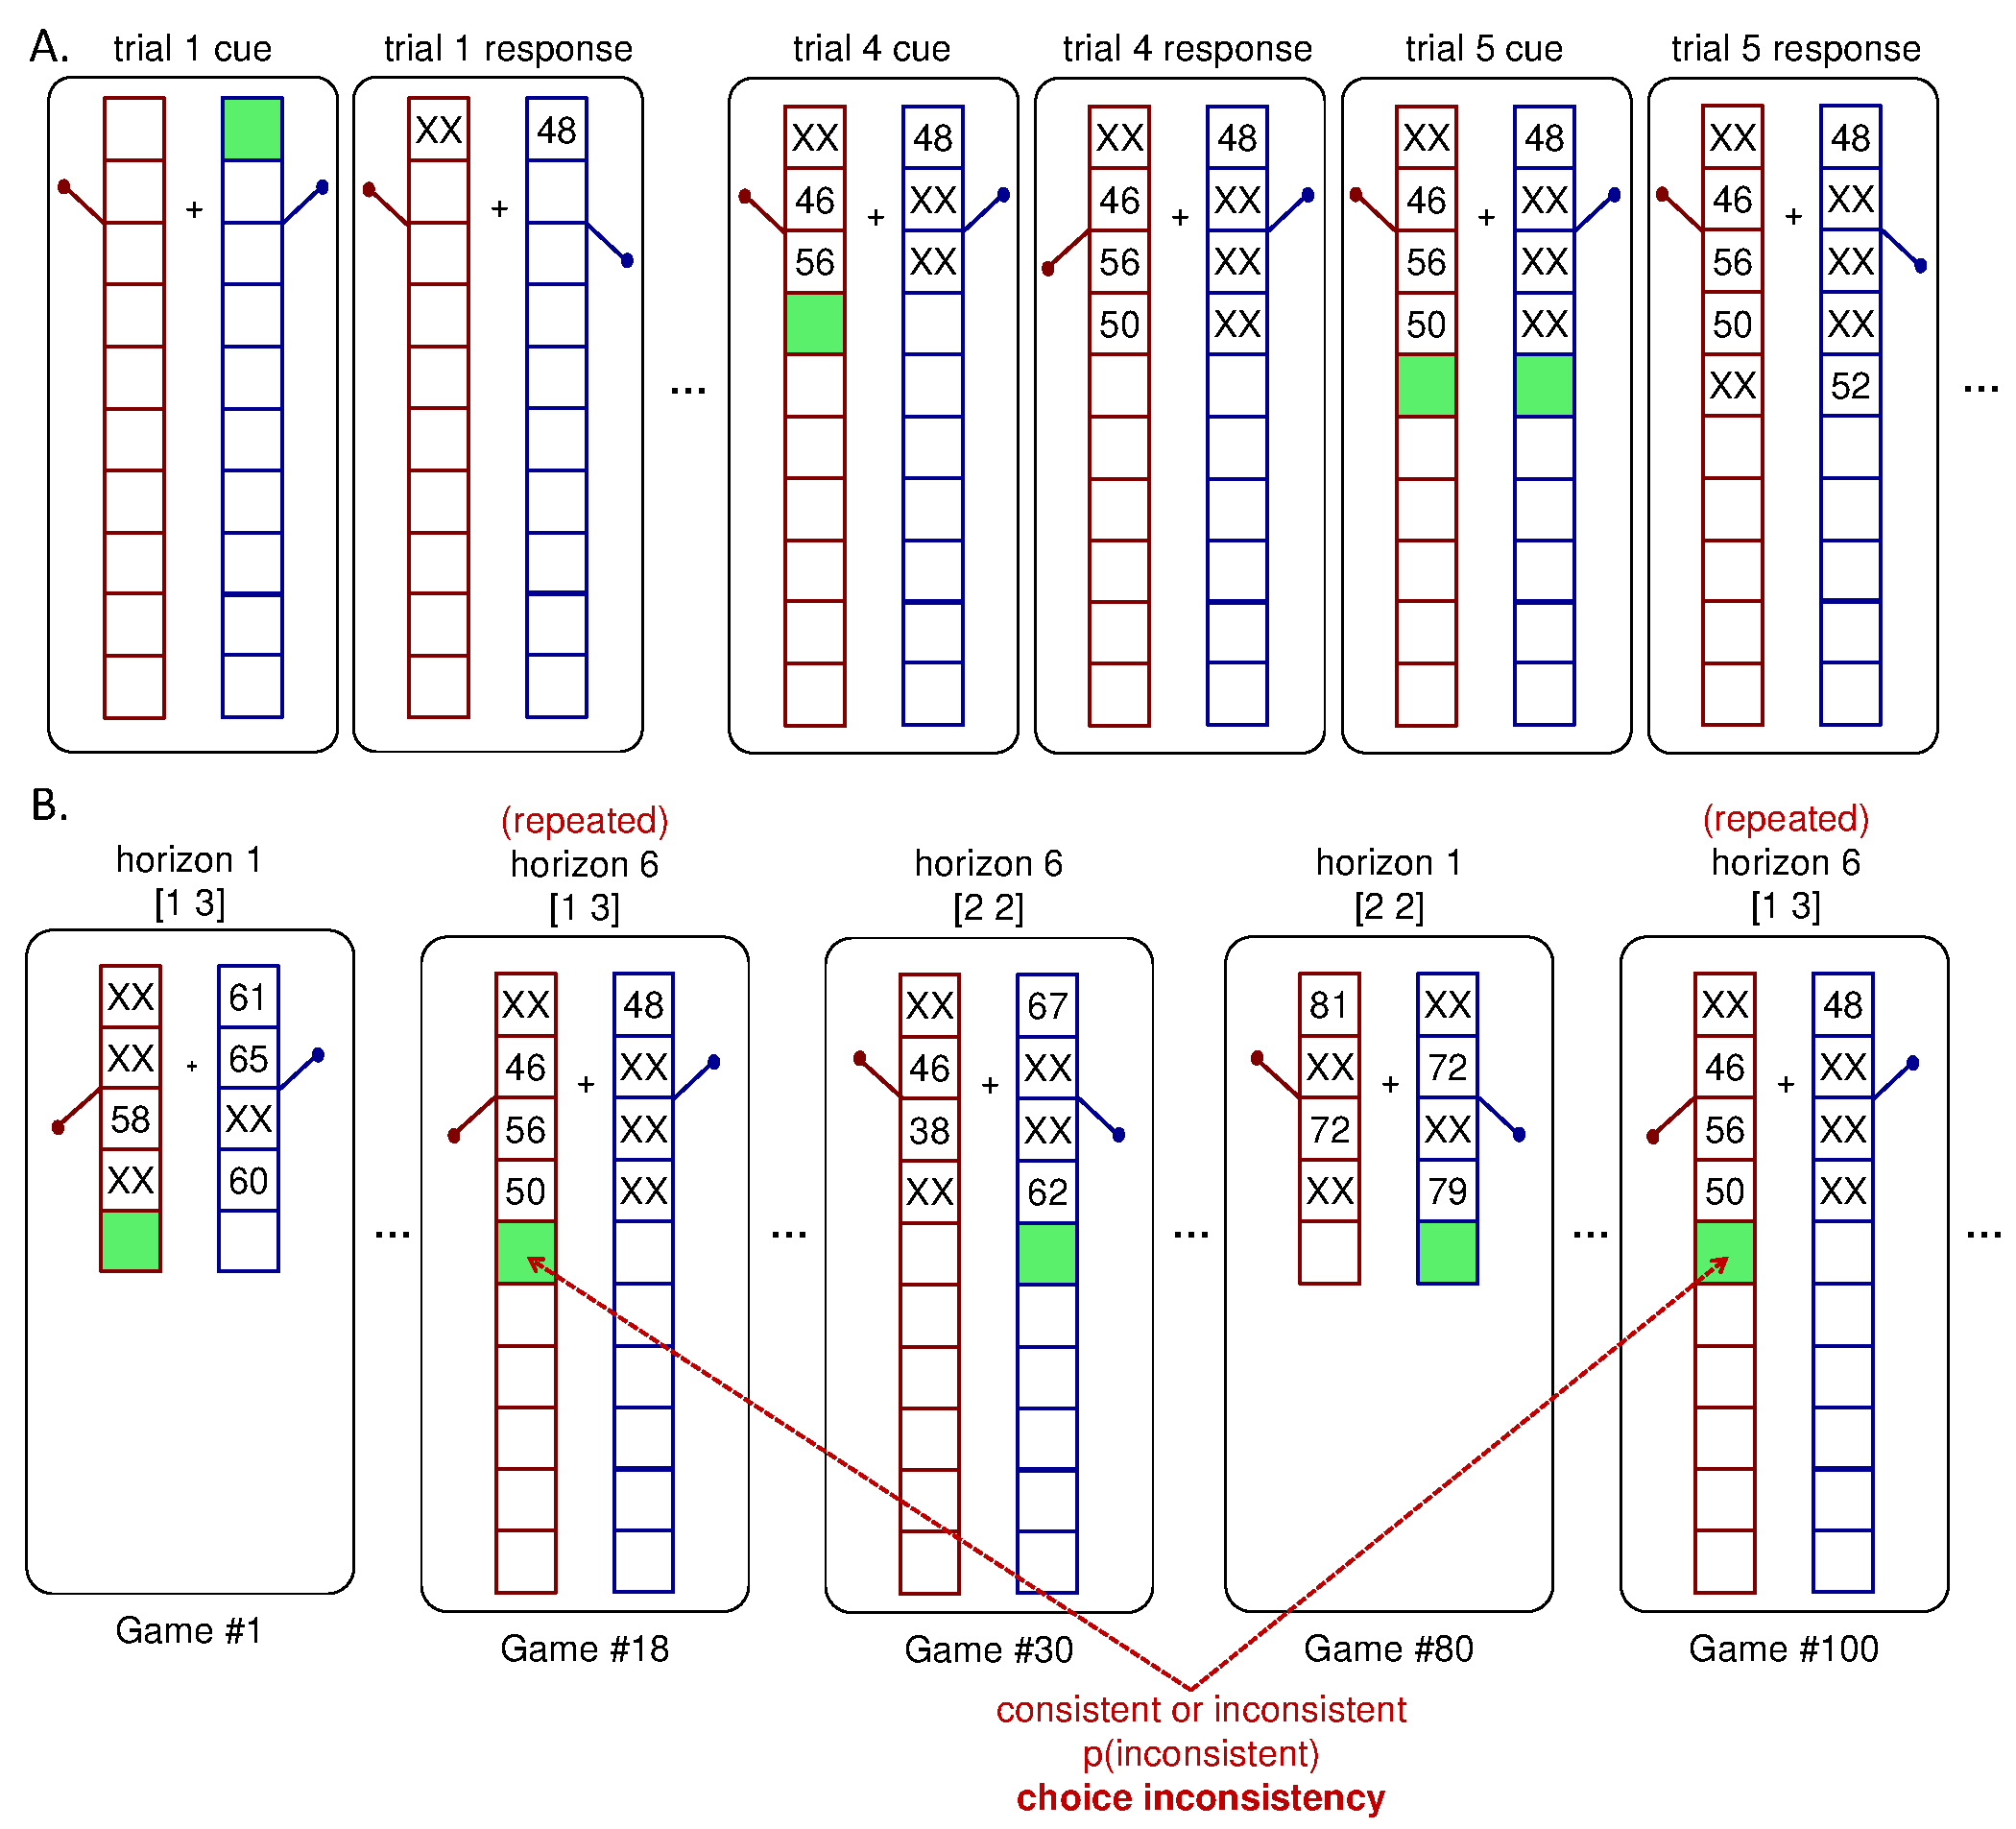
\includegraphics[width=\textwidth]{figures/taskfiga.pdf}
			\caption{ 
				Schematic of the experiment. (A) Dynamics of an example horizon 6 game.  Here the first four trials are forced trials in which participants are instructed which option to play.  After the forced trials, participants are free to choose between the two options for the remainder of the game.  (B) Example repeated games over the course of the experiment.
				% Different possible states of the game after the first free choice over the course of the experiment. 
				On average, participants play more than 150 such games, with varying horizon (1 vs 6), uncertainty condition ([1 3] vs [2 2]) and observed rewards.  In addition, all games are repeated (as Game 18 and 100 are here) such that participants will be faced with the exact same pattern of forced trials and exact same outcomes from those forced trials twice within each experiment.  These repeated games allow us to compute the relative contribution of deterministic and random noise by analyzing the extent to which choices are {\em consistent} across the repeated games.}
			\label{fig:taskfig}
		\end{center}
	\end{figure}
	
	The task is organized in games (Figure \ref{fig:taskfig}A). The mean payout of the two bandits are held fixed within a game and reset between games. Each game consists of either 5 or 10 trials. The first four trials of each game are `forced-choice' trials. In the first four trials, participants are instructed about which bandit to choose, this allows us to manipulate what information from both bandits participants receive before they make their first free choice between the two bandits. From the 5th trial, participants make free choices between the two bandits. Participants have either 1 or 6 free choices to make. 
	
	The Horizon Task has two key features that together allow it to quantify explore-exploit behavior. The first of these features is  the time horizon --- the number of decisions participants will make in the future. By changing this horizon from short (1 free-choice trial) to long (6 free-choice trials), the Horizon Task allows us to control the relative value of exploration and exploitation. Just like the restaurant example in the introduction, when the horizon is short, participants should be more likely to exploit the option they believe to be best, because this leads to the highest payoff in the short term. Conversely, when the horizon is long, participants should be more likely to explore at first, because this allows them to gather information to make better choices later on. By contrasting behavior between short and long horizon conditions {\it on the very first free-choice trial}, when all else is equal, the Horizon Task allows us to quantify how behavior changes, when it is more valuable to explore.
	
	The second key feature of the Horizon Task are the 4 forced-choice trials at the start of each game that allow us to control exactly what participants know about the two bandits before they make their choice. In these forced-choice trials, participants are instructed which of the bandits to play allowing us to control how much information they have about each of the options. The forced-choice trials are used to set up one of two information conditions: an `unequal information' or [1 3] condition, in which participants play one bandit once and the other three times, and an `equal information' or [2 2] condition, in which participants play both bandits twice.
	
	Relative to the original Horizon Task, the key modification in this paper is to give people `repeated games' (Figure \ref{fig:taskfig}B), in which they see the exact same set of forced-choice plays twice in two separate games separated by several minutes in time so as to avoid detection. By repeating the forced-choice plays for each game twice, we can set up a situation where (unbeknownst to the participants) they are faced with the exact same explore-exploit choice, with the exact same stimuli twice. Thus, if their behavior is a deterministic function of the stimuli, then they will make the same decision in both games and their choices will be consistent. Conversely, if their behavior is not driven by a deterministic function of the stimulus, then their choices on the repeated games will be inconsistent some fraction of the time. The extent to which participants' choices are consistent on the repeated versions of the games allow us to quantify the extent to which the variability in their behavior was driven by a deterministic process vs a random noise process.
	
	\subsection*{Both behavioral variability and information seeking increase with horizon}
	Before discussing the results for repeated games, we first confirm that the basic behavior in this task is consistent with our previously reported results using both a model-free and model-based approach \citep{wilson2014}. In both analyses, we focus on just the first free-choice trial in each game, where the only thing that differs between the horizon conditions is the number of choices that participants will make in the future. 
	
	\subsubsection*{Model-free analysis}
	In the model-free analysis, we quantify random and directed exploration using simple choice probabilities. Random exploration is quantified as the probability of choosing the option that has the lower average payout in the forced-choice plays in the equal, or [2 2], condition, $p(\mbox{low mean})$. The idea here is that, in the equal condition, the optimal strategy is to compute the mean payout for each bandit from the forced-choice plays and then always choose the option with the highest mean. When participants do not choose the option with the higher mean, the assumption is that this is due to some kind of `decision noise', making the probability of choosing the low mean option a measure of behavioral variability. In this view, random exploration corresponds to an increase in $p(\mbox{low mean})$ with horizon, which is exactly what we see in the data (Figure \ref{fig:modelfree}A; t(64) = 7.99, p $<$ 0.001).
	
	Directed exploration is quantified as the probability of choosing the more informative option $p(\mbox{high info})$ in the unequal, or [1 3], condition. The more informative option is the option played once during the forced-choice plays as choosing this option gives relatively more information (doubling the number of samples from 1 to 2) than choosing the option played three times (only increasing the number of sample by a third, from 3 to 4). In this view, directed exporation corresponds to an increase in $p(\mbox{high info})$ with horizon, which is exactly what we see in the data (Figure \ref{fig:modelfree}B; t(64) = 6.92, p $<$ 0.001).
	
	\subsubsection*{Model-based analysis}	
	Another approach to understanding behavior in the Horizon Task is to use a computational model \citep{wilson2014}. In this case, we model  participants' choices on the first free-choice trial by assuming they make decisions by computing the difference in value (or utility) $\Delta Q$ between the right and left options, choosing right when $\Delta Q > 0$ and left otherwise.  Specifically, we write
	\begin{equation}
		\label{eq:origmodel}
		\Delta Q= \Delta R+A \Delta I+b+n
	\end{equation}
	where, the experimentally controlled variables are $\Delta R=R_{right}-R_{left}$, the difference between the mean of rewards shown on the forced-choice trials, and $\Delta I$, the difference in information available for playing the two options on the first free-choice trial. For simplicity, and because information is manipulated categorically in the Horizon Task, we define $\Delta I$ to be +1 if one reward is drawn from the right option and three are drawn from the left in the [1 3] condition, -1 if one from the left and three from the right in the [1 3] condition, and in [2 2] condition, $\Delta I$ is 0. 
	
	Here, $n$ denotes decision noise, which, in this version of the model is a combination of deterministic and random noise. $n$ is assumed to come from a logistic distributions with mean 0 and standard deviations $\sigma$.
	
	The free parameters of this model are: the information bonus $A$, which controls the level of directed exploration; the noise standard deviation, $\sigma$, which controls the level of random exploration, and the spatial bias, $b$, which determines the extent to which participants prefer the option on the right. These free parameters are fit separately for each participant in each horizon condition, allowing us to test whether directed and random exploration increase with horizon. Consistent with previous research, we find that this is indeed the case (Figure \ref{fig:modelfree}C; t(64) = 5.35, p $<$ 0.001. Figure \ref{fig:modelfree}D; t(64) = 3.54, p $<$ 0.001). 
	
	\begin{figure}[H]
		\begin{center}
			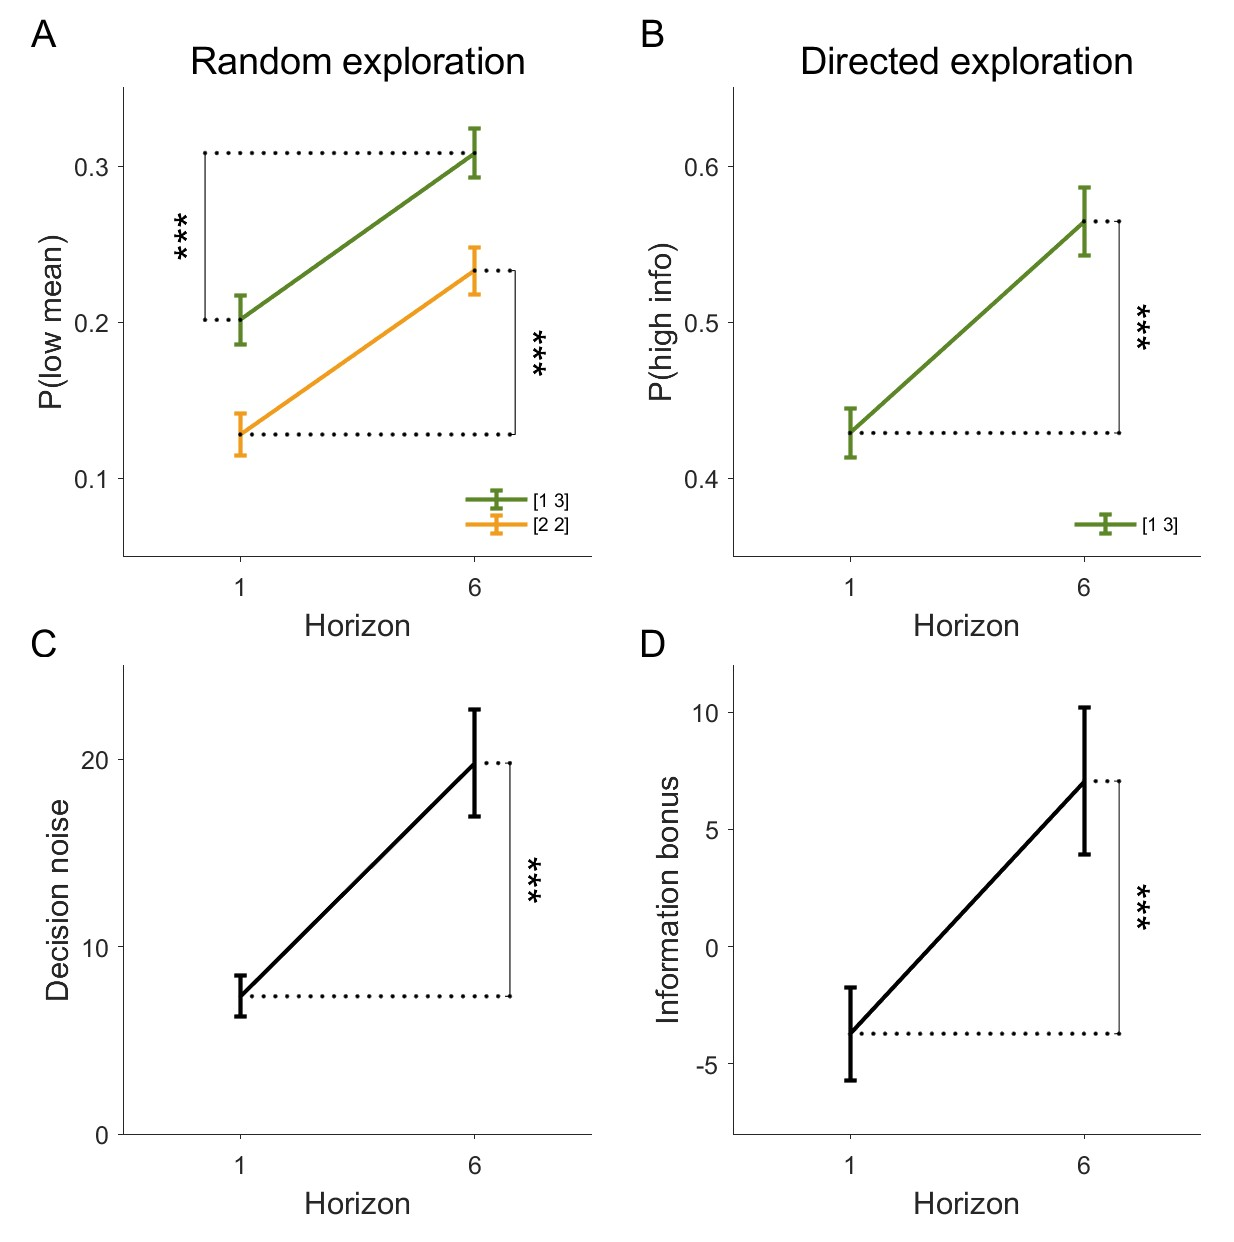
\includegraphics[width=\textwidth]{figures/RanDetNoise_modelfree.jpg}
			\caption{Replication of previous findings that people use both random and directed exploration in this task. (A) model-free measure of behavioral variability, $p(\mbox{low mean})$, increases with horizon. (B) model-free measure of information seeking, $p(\mbox{high info})$, increases with horizon. (C) model-based measure of behavioral variability, decision noise $\sigma$, increases with horizon. (D) model-based measure of information seeking, information bonus $A$, increases with horizon.}
			\label{fig:modelfree}
		\end{center}
	\end{figure}
	
	Taken together, our model-free and model-based analyses agree with previous findings showing increased behavioral variability and increased information seeking in the long horizon condition, consistent with humans using random and directed exploration (Figure \ref{fig:modelfree}, Supplementary Figure S1). However, for random exploration, this previous analysis cannot distinguish between deterministic and random sources of noise. For this we analyze the extent to which people's choices are consistent on the repeated games.
	
	
	%  In this analysis, random exploration is quantified in a model-free way as the probability of choosing the option that has the lower average payout in the example plays in the equal, or [2 2], condition, $p(\mbox{low mean})$. The idea here is that in the equal condition, the optimal strategy is to compute the average payout for each bandit from the example plays and then always choose the option with the highest average. When participants do not choose the higher average option, the assumption is that this is due to some kind of `decision noise.' In this view, random exploration corresponds to an increase in $p(\mbox{low mean})$ with horizon, which is exactly what we see in the data (Figure \ref{fig:modelfree}A; t(64) = 6.55, p $<$ 0.001 for [1 3], t(64) = 7.99, p $<$ 0.001 for [2 2]).}

	% Directed exploration, is measured as the probability of choosing the more informative option $p(\mbox{high info})$ in the unequal, or [1 3], condition. Again this measure increases with horizon, showing that people are more information seeking in horizon 6 than horizon 1 (t(64) = 6.92, p $<$ 0.001).  \added[id=bob]{Together, these results are consistent with the idea that people use both random exploration and directed exploration and increase both behavioral variability and information seeking when the time horizon is long.}


\subsection*{Model-free analysis of repeated games suggests that random exploration involves both random and deterministic noise}

Next we asked whether participants' choices were consistent or inconsistent in the two repetitions of each game. The idea behind this measure is that purely deterministic noise should lead to consistent choices as the deterministic stimulus is identical both times. Conversely, if choice is not entirely driven by a deterministic process and is also driven by random noise, participants' choices should be more inconsistent across the repetitions of the game. Moreover, if decision noise is purely random noise, meaning there is no unobserved deterministic process, we will show that we can actually predict the expected level of choice inconsistencies across repetitions of games by accounting for the known deterministic processes and assuming that the random noise process is independent in repetitions of the game.

To quantify choice inconsistency we computed the frequency with which participants made different responses for pairs of repeated games (Figure \ref{fig:mf2}, Supplementary Figure S2). Using this measure we found that participants made inconsistent choices in both the unequal ([1 3]) and equal ([2 2]) information conditions ($p(\mbox{inconsistent}) > 0 $), suggesting that not all of the noise was stimulus driven. In addition, we found that choice inconsistency was higher in horizon 6 than in horizon 1 for both [1 3] and [2 2] condition (For [1 3] condition, t(64) = 5.41, p $<$ 0.001; for [2 2] condition, t(64) = 6.26, p $<$ 0.001), suggesting that at least some of the horizon dependent noise is not a deterministic function of the stimulus, but rather random noise.

% (t-test vs zero revealed that inconsistency was greater than zero for all horizon and uncertainty conditions)

%\deleted[id=siyu]{For [1 3] condition, t(64) = 13.72, p $<$ 0.001 for horizon 1, t(64) = 16.71, p $<$ 0.001 for horizon 6; For [2 2] condition, t(64) = 9.55, p $<$ 0.001 for horizon 1, t(64) = 17.93, p $<$ 0.001 for horizon 6}
\begin{figure}[H]
	\begin{center}
		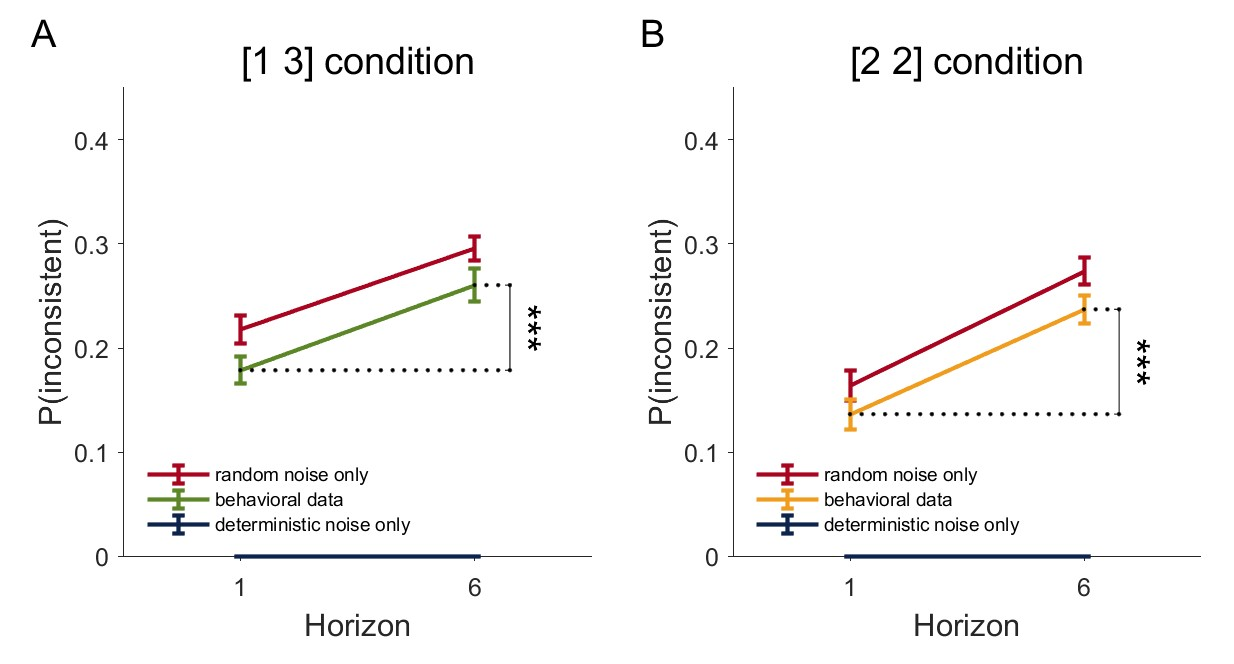
\includegraphics[width=\textwidth]{figures/RanDetNoise_pinconsistent.jpg}
		\caption{Model-free analysis suggests that both deterministic and random noise contribute to the choice variability in random exploration. For both the [1 3] (A) and [2 2] (B) condition, people show greater choice inconsistency in horizon 6 than horizon 1. However, the extent to which their choices are inconsistent lies between what is predicted by purely deterministic and random noise, suggesting that both noise sources influence the decision.}
		\label{fig:mf2}
	\end{center}
\end{figure}

To gain more quantitative insight into these results, we computed theoretical values for the choice inconsistency for the purely deterministic and purely random noise cases.  For purely deterministic noise this computation is simple because people should make the exact same decisions each time in repeated games, meaning that $p(\mbox{inconsistent}) = 0$ in this case. For purely random noise, the two games should be treated independently, allowing us to compute the choice inconsistency in terms of the probability of choosing the low mean option, $p(\mbox{low mean})$, as
\begin{equation*}
	\begin{split}
		p(\mbox{consistent}) &= p(\mbox{low mean})^2 + p(\mbox{high mean})^2\\
		&= p(\mbox{low mean})^2 + (1-p(\mbox{low mean}))^2\\ 
		\mbox{hence},\quad p(\mbox{inconsistent}) &=  
		1 - p(\mbox{consistent}) = 
		2 p(\mbox{low mean})(1-p(\mbox{low mean}))
	\end{split}
\end{equation*}

Furthermore, to account for the fact that $p(\mbox{low mean})$ is a function of reward difference $\Delta R$ between the two bandits and the information condition $I$, we estimated the conditional probability:
	$$p(\mbox{inconsistent}|\Delta R, I) = 2 p(\mbox{low mean}|\Delta R, I)(1-p(\mbox{low mean}|\Delta R, I))$$
	Then based on the likelihood that each condition ($\Delta R$ and $I$) occurs in the task $\rho(\Delta R, I)$, we have
	$$p(\mbox{inconsistent}) = \sum_{\Delta R, I}\rho(\Delta R, I)p(\mbox{inconsistent}|\Delta R, I)$$

As shown in Figure \ref{fig:mf2}, people's behavior falls in between the pure deterministic noise prediction and the pure random noise prediction. Specifically, behavior is different from the pure random noise prediction in the both the [1 3] condition (t(64) = 4.83, p $<$ 0.001 for horizon 1, t(64) = 3.12 p $=$ 0.003 for horizon 6) and the [2 2] condition (t(64) = 3.92, p $<$ 0.001 for horizon 1, t(64) = 3.71, p $<$ 0.001 for horizon 6). Likewise, behavior is different from pure deterministic noise prediction in both the [1 3] condition (t(64) = 13.72, p $<$ 0.001 for horizon 1, t(64) = 16.71, p $<$ 0.001 for horizon 6) and the [2 2] condition (t(64) = 9.55, p $<$ 0.001 for horizon 1, t(64) = 17.93, p $<$ 0.001 for horizon 6). As a negative control of our method for estimating $p(\mbox{inconsistent})$ for purely random noise, we simulated choices using a decision model that only includes random noise (Equation \ref{eq:newmodel}), and found that $p(\mbox{inconsistent})$ in this simulated data is not different from our pure random noise prediction in all horizon and uncertainty conditions (p $>$ 0.05, Supplementary Figure S3). Together, our results suggest that both random noise and deterministic noise contribute to the choice variability in random exploration. However, the relative contribution from each of these types of noise, as well as how each type of noise changes with horizon, are difficult to discern.

\subsection*{Model-based analysis provides a lower-bound estimate of deterministic noise and an upper-bound estimate of random noise}

To more precisely quantify the contribution of deterministic noise and random noise, we turned to model fitting. We modeled behavior on the first free choice of the Horizon Task using a version of the logistic choice model (Equation \ref{eq:origmodel}) that was modified to differentiate between components of the noise that are deterministically driven by the stimulus (`deterministic noise') and components of the noise that are not deterministically driven by the stimulus (`random noise'). In particular, we assume that in repeated games, the value of stimulus-driven deterministic noise is frozen whereas random noise is drawn independently both times. 

\subsubsection*{Overview of model}
%As with our model-free analysis, the model-based analysis focuses only on the first free-choice trial since that is the only free choice when we have control over the experience participants have about two bandits. 
To model participants' choices on the first free-choice trial, we use a modified version of Equation \ref{eq:origmodel}.
%assume that they make decisions by computing the difference in value $\Delta Q$ between the right and left options, choosing right when $\Delta Q > 0$ and left otherwise.  Specifically, we write
\begin{equation}
	\label{eq:newmodel}
	\Delta Q= \Delta R+A \Delta I+b+n_{det}+n_{ran}
\end{equation}
where, as before $\Delta R$, is the the difference in mean rewards shown on the forced-choice trials, $\Delta I$, is the difference in information, $A$ is the information bonus, and $b$ is the spatial bias. New in Equation \ref{eq:newmodel} are the terms $n_{det}$ and $n_{ran}$. $n_{det}$ denotes the deterministic noise, which is identical on the repeat versions of each game; and $n_{ran}$ denotes random noise, which is uncorrelated between repeated plays and changes every game. $n_{det}$ and $n_{ran}$ are assumed to come from logistic distributions with mean 0, and standard deviations $\sigma_{det}$ and $\sigma_{ran}$. 

%The subject-and-condition-specific parameters are: the spatial bias, $b$, which determines the extent to which participants prefer the option on the right; the information bonus $A$, which controls the level of directed exploration; 

For each pair of repeated games, the set of forced-choice trials are exactly the same, so the deterministic noise, $n_{det}$, should be the same while the random noise, $n_{ran}$ may be different. This is exactly how we distinguish deterministic noise from random noise. In symbolic terms, for repeated games $i$ and $j$,  $n_{det}^i=n_{det}^j$  and $n_{ran}^i \neq n_{ran}^j$.

We used hierarchical Bayesian analysis to fit the parameters of the model (see Figure \ref{fig:model} for a graphical representation of the model in the style of \cite{lee2014}). In particular, we fit values of the information bonus $A$, spatial bias $b$, variance of random noise $\sigma_{ran}^2$, and variance of deterministic noise $\sigma_{det}^2$ for each participant in each horizon. Model fitting was performed using the MATJAGS and JAGS software \citep{jags, matjags} with full details given in the Methods.  

\subsubsection*{Model validation}
To be sure that our fit parameter values were meaningful and to understand the limits of our model, we evaluated our model extensively using simulated data. This allowed us to quantify whether deterministic and random noise can be identified under ideal conditions where the behavior is generated by the model with known parameters. Full details are presented in the Supplementary Materials section 2. 
	
In this section we focus on our results for parameter recovery \citep{Wilson2019}. In a parameter recover analysis, behavioral data is simulated by the model with known parameters and then this simulated behavioral data is fit with the model to quantify the extent to which fit parameters match the input simulated parameters --- that is, whether the simulated parameters can be recovered.  
	
\begin{figure}[H]
	\begin{center}
		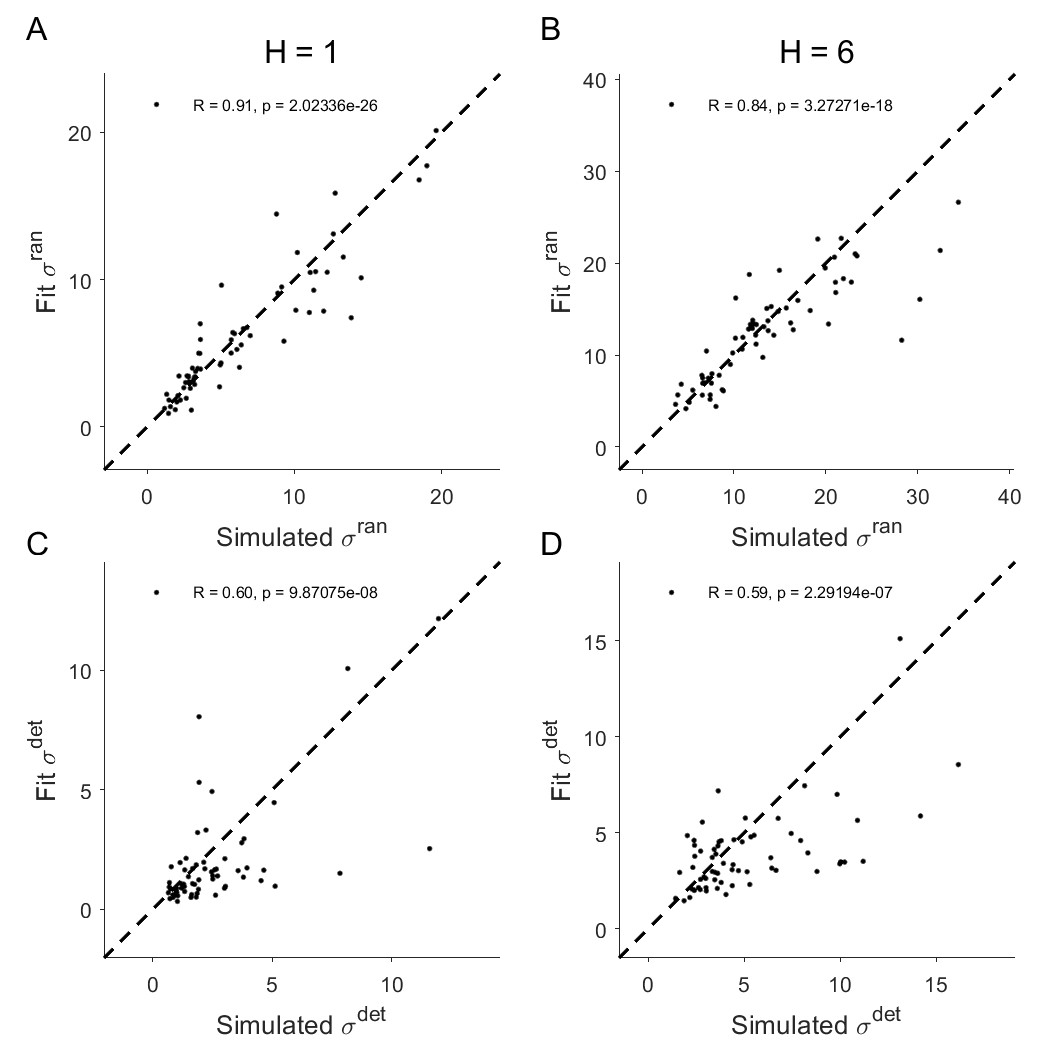
\includegraphics[width=.95\textwidth]{figures/RDBayes_parameterrecovery_subject_examplesession_randet.jpg}
		\caption{Parameter recovery analysis for random (A,B) and deterministic (C,D) noises in the two horizons.}
		\label{fig:paramrecover_main}
	\end{center}
\end{figure}

Parameter recover in this task was good for this model, with fit values for $\sigma_{ran}$ and $\sigma_{det}$ showing strong correlations with their simulated values in both horizon (H) conditions (For $\sigma_{ran}$, $R = 0.91 (\mbox{H} = 1) \mbox{ and } 0.84 (\mbox{H} = 6), p < 0.001$, For $\sigma_{det}$, $R = 0.60 (\mbox{H} = 1) \mbox{ and } 0.59 (\mbox{H} = 6), p < 0.001$). However, while the relationship was near perfect for random noise ($\frac{\mbox{\small Recovered } \sigma_{ran}}{\mbox{\small Simulated } \sigma_{ran}} = 1.01$), there was a systematic bias to underestimate the level of deterministic noise by about 32\% ($\frac{\mbox{\small Recovered } \sigma_{det}}{\mbox{\small Simulated } \sigma_{det}} = 0.68$). Despite this underestimation of deterministic noise in both horizon conditions, the difference in deterministic noise between horizons is much better captured (see Supplementary Materials section 2.2). This is because the underestimation of deterministic noise is partially canceled out when the difference is taken between horizon conditions. In addition, we see better parameter recovery for random noise than deterministic noise. This is likely because we effectively have half as many trials for deterministic noise. In particular, while we generate two samples of random noise for each repeated game pair, we only generate one sample of deterministic noise, which by definition is the same in both of the repeated games. 
	% $\frac{\mbox{\small Recovered } \Delta \sigma_{det}}{\mbox{\small Simulated } \Delta \sigma_{det}} = 0.74$
	
In addition to the conventional subject-level parameter recovery analysis presented here, we also performed parameter recovery analysis that examined how faithful the full posterior distribution of group-level parameters can be recovered in simulated data (Supplementary Figure S5, S6). Qualitatively, we also showed that our way of modeling deterministic noise is capable of capturing known deterministic processes intentionally omitted from the full model (Supplementary Figure S4). Full details of these additional analysis are presented in the Supplementary Materials. 
		
Overall, we were able to detect both deterministic and random noises using our model. Because random noise is modeled as non-stimulus-driven noise, it can reflect both true stochastic random noise and possible deterministic noises which do not depend on the stimuli. Thus conceptually our random noise estimate provides an upper bound for the true `random noise' induced by intrinsic stochastic processes in the brain. Thus, our model provides a lower bound for deterministic noise and an upper bound for random noise. 

\subsubsection*{Model-based results} 
Posterior distributions over the group-level means of the deterministic and random noise standard deviation $\sigma_{det}$ and $\sigma_{ran}$ are shown in Figure \ref{fig:mb1} and Supplementary Figure S11. Consistent with our model-free results, we see that both random and deterministic noise are non-zero. Numerically, random noise is about 2-3 times larger than the deterministic noise. By computing the posterior distribution of $\sigma^2_{det}/(\sigma^2_{det}+\sigma^2_{ran})$, our data suggests that 14.25\% of the variability in random exploration is accounted for by deterministic noise ([4.90\%, 28.81\%], 95\% CI). In addition, we find that both random and deterministic noise increase with horizon. This increase was larger for random noise (mean = 7.13, 100\% of samples showed an increase in random noise with horizon) than deterministic noise (mean = 2.59, 98.64\% of samples showed an increase in deterministic noise with horizon). But intriguingly, the relative increase in both types of noise was similar (Figure \ref{fig:ratio}). That is, when we compute the relative increase in deterministic noise with horizon, $\sigma^{det}_{horizon6}/\sigma^{det}_{horizon1}$, it is very similar to the relative increase in random noise with horizon $\sigma^{ran}_{horizon6}/\sigma^{ran}_{horizon1}$. 

\begin{figure}[H]
\begin{center}
	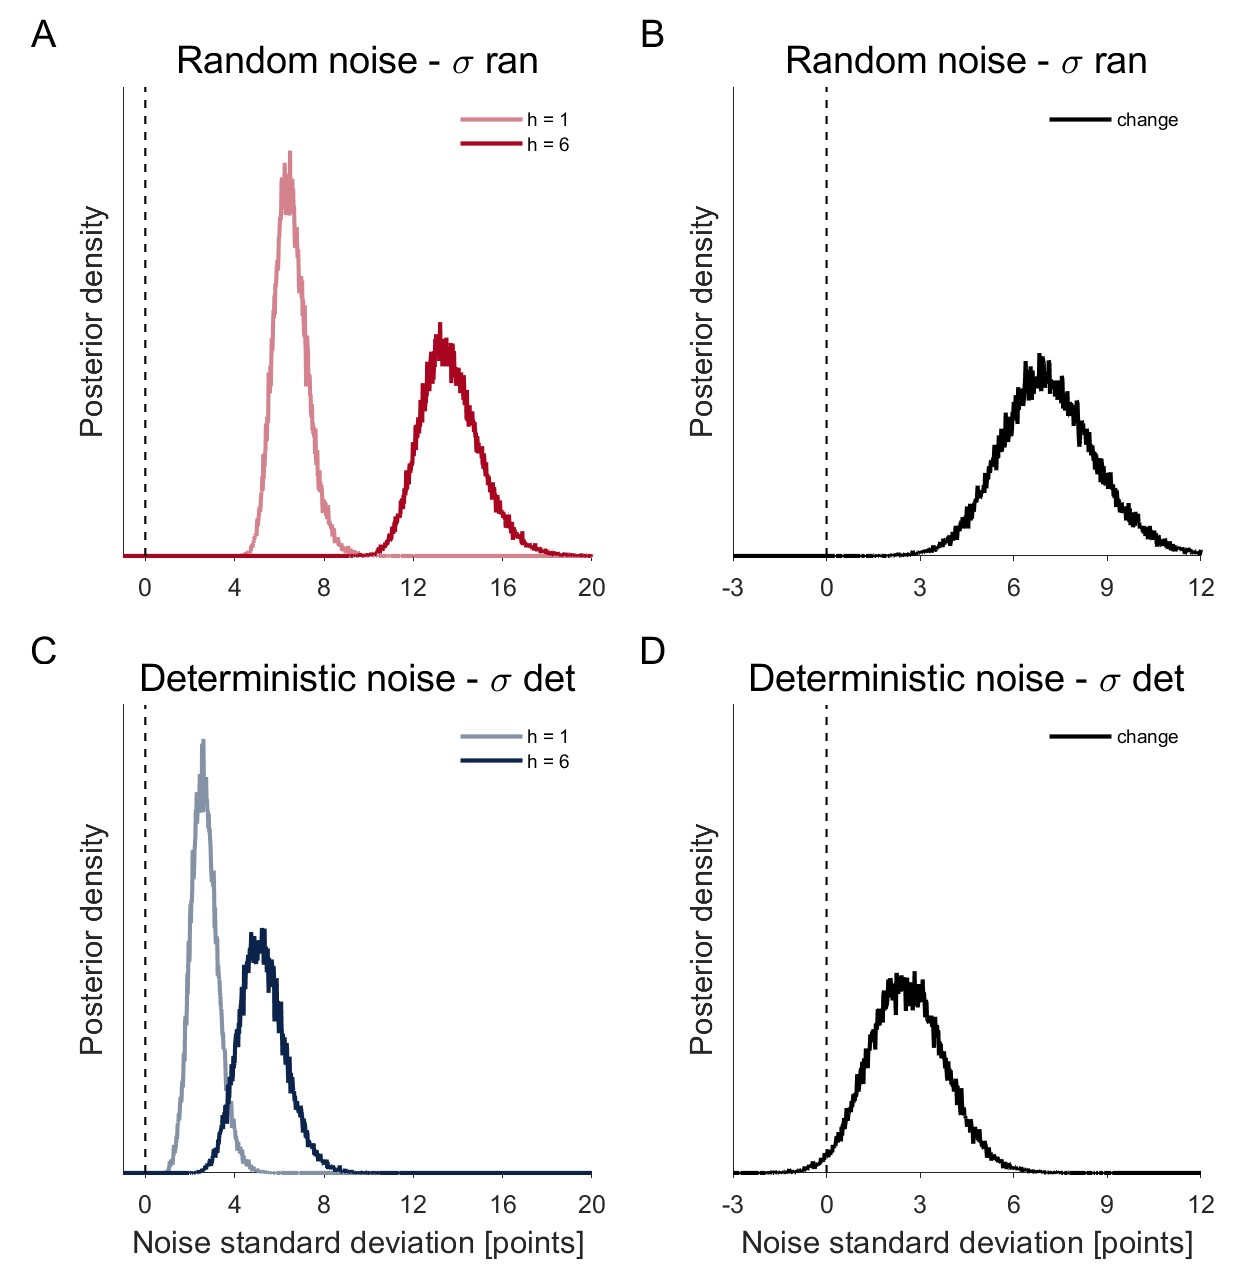
\includegraphics[width=\textwidth]{figures/RDBayes_hyperprior.jpg}
	\caption{Model based analysis showing the posterior distributions over the group-level mean of the standard deviations of  random and deterministic noise. Both random (A, B) and deterministic (C,D) noises are nonzero (A, C) and increase with horizon (B, D).  }
	%BOB SAYS: However, random noise has both a greater magnitude overall (A, C) and a greater change with horizon (B, D) than deterministic noise.
	\label{fig:mb1}
\end{center}
\end{figure}

\begin{figure}[H]
\begin{center}
	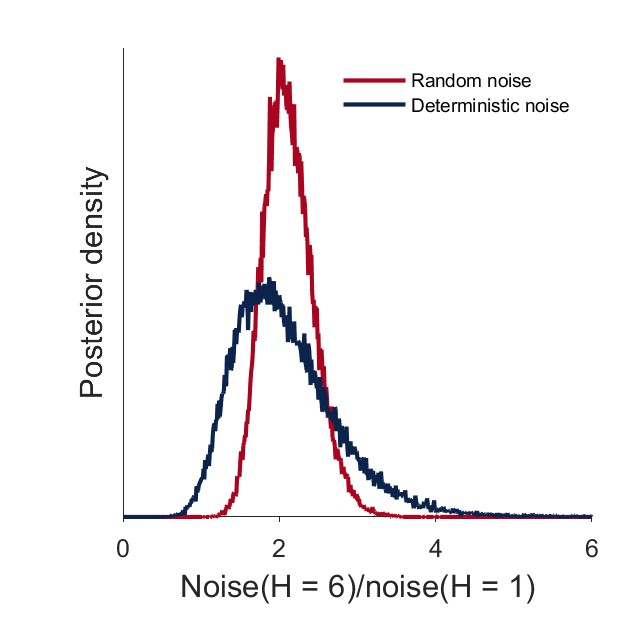
\includegraphics[width=0.5\textwidth]{figures/RDBayes_ratio.jpg}
	\caption{Model based analysis showing the posterior distributions over the ratio of the group-level mean of the standard deviations of  random and deterministic noise between horizon 6 and horizon 1 respectivelly. The ratios in the standard deviations of noises between horizon 6 and horizon 1 are similar for random and deterministic noise.}
	\label{fig:ratio}
\end{center}
\end{figure}

\subsubsection*{Posterior predictive checks}
In addition to fitting the model to behavior, it is also important to check whether the model captures the qualitative patterns of the data \citep{Wilson2019} --- specifically how p(high info), p(low mean) and p(inconsistent) change with horizon.

To perform this `posterior predictive check', we created a set of simulated data by taking the subject-level parameters from the hierarchical Bayesian fits and having the model play the same sequence of games as seen by the subjects. We then applied the same model-free analysis as described in the previous sections to this simulated data set and compared the model's behavior to that of participants. As shown in Figure \ref{fig:mb3}, the model can account for all qualitative patterns in the data --- the increase in p(high info), p(low mean), and p(inconsistent) with horizon, and that p(inconsistent) is in between pure random and pure deterministic noise. The quantitative agreement is almost perfect for p(high info) and for p(inconsistent) in the [1 3] condition, but the model seems to systematically overestimate p(low mean) and p(inconsistent) in [2 2] conditions, although the discrepancy is relatively small (overestimating p(low mean) by 0.054 or 31.37\%, and p(inconsistent) by 0.049 or 27.83\% in [2 2] condition). 

As a control, we also applied posterior predictive checks on alternative models that consider only deterministic or only random noise, and these reduced models fail to capture all qualitative patterns (Supplementary Figure S13). Full details of this analysis can be found in Supplementary Materials section 3.2.  

\begin{figure}[H]
\begin{center}
	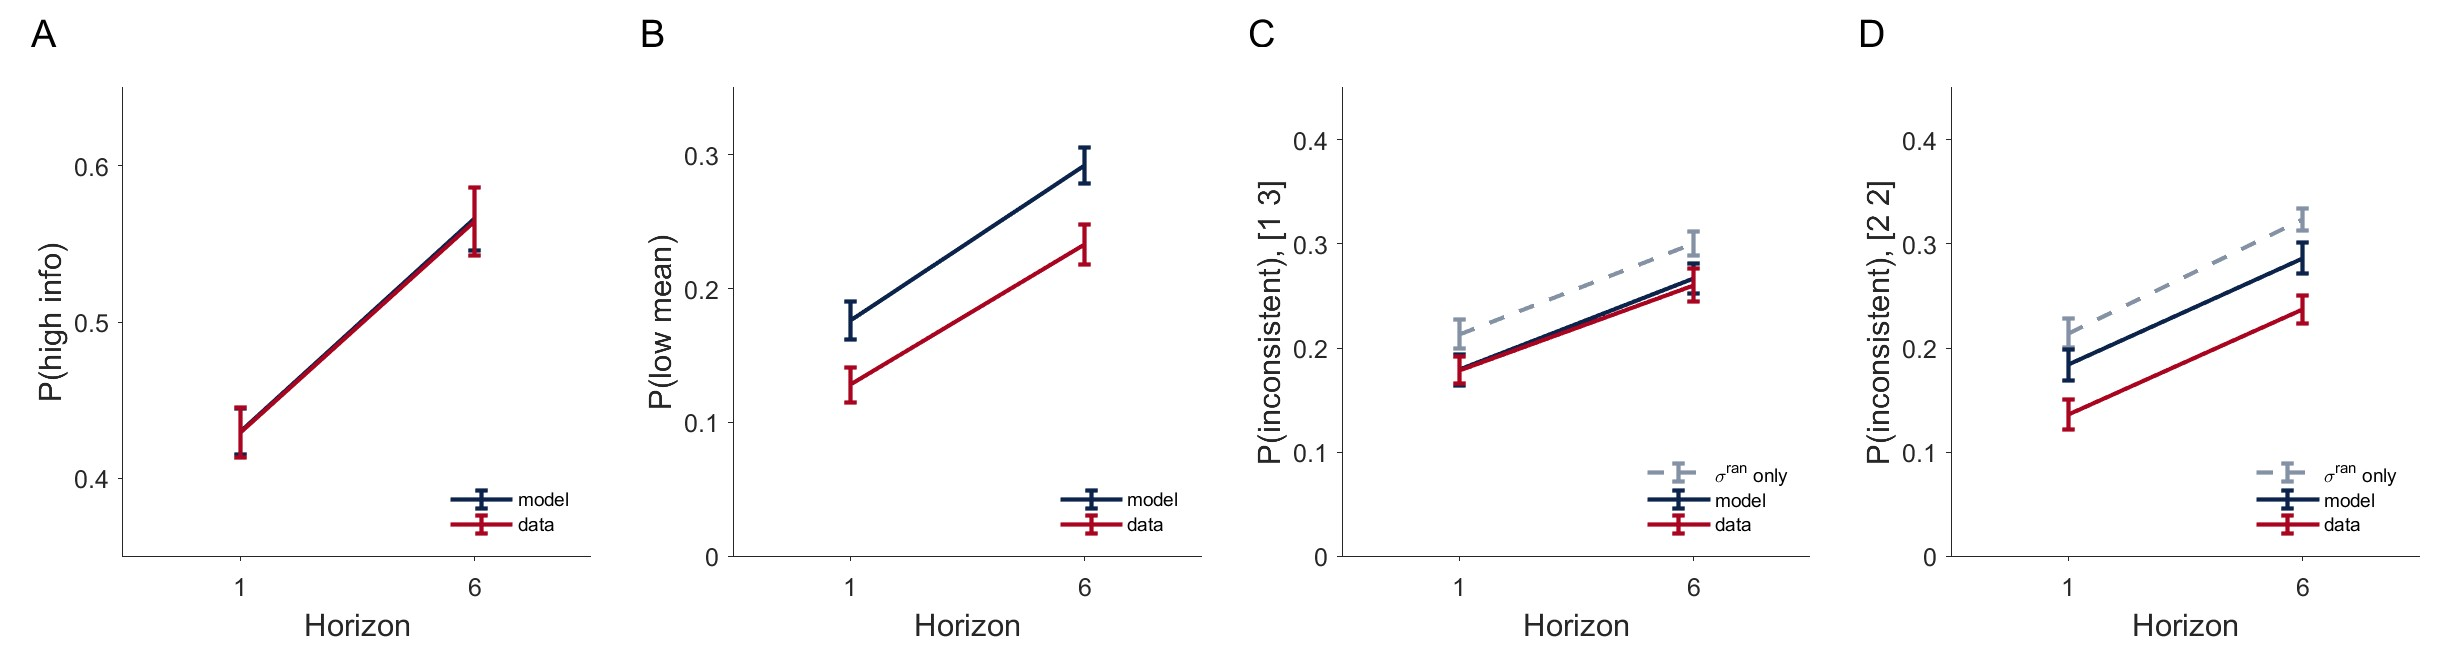
\includegraphics[width=1\textwidth]{figures/RDBayes_2noise_modelA.jpg}
	\caption{
		Our model accounts for all qualitative patterns of the data, namely, (A) p(high info) and (B) p(low mean) increase as a function of horizon, p(inconsistent) increases as a function of horizon for both [1 3] (C) and [2 2] (D) conditions and it lies between the pure random and pure deterministic noise prediction.}
	\label{fig:mb3}
\end{center}
\end{figure}


%dominated by random noise. To test this more explicitly, we build a series of models in which different assumptions are made regarding the presence and absence of both types of noise and whether each type of noise if exists is horizon dependent (See Table \ref{tab:models}). In model A-D, we assumed the existence of both random and deterministic noise, in model A and B, random noise is assumed to be horizon-dependent, whereas in model A and C, deterministic noise is assumed to be horizon dependent. In model E, we assumed no random noise. In model F, we assumed no deterministic noise. 

%To evaluate and compare between models, we simulated choice behavior by taking the subject-level parameters from the Hierarchical Bayesian fits. The same model-free analysis as described in the previous session is applied to all 6 sets of simulated data for the 6 models respectively. (See Figure  \ref{fig:mb3}). 

%The original measure of random exploration, p(low mean), as used in \cite{wilson2014} can be explained by having deterministic noise alone (Figure \ref{fig:mb3}, Panel E2) or having random noise alone (Figure \ref{fig:mb3}, Panel F2). That participants qualitatively exploit the high-mean option less and choose the low-mean option more in horizon 6, can be explained by having both pure deterministic noise and pure random noise, as long as noise is horizon dependent. If both deterministic and random noise are assumed to be the same for both horizons (Figure \ref{fig:mb3}, Panel D), p(low mean) becomes completely flat and no horizon dependent random exploration is observed.

%On the other hand, by looking at the percentage of inconsistent choices in the repeated pair of game, p(inconsistent), external noise alone can not account for behavior any more (Figure \ref{fig:mb3}, Panel E3, E4). Moreover, model C and D are disqualified that the increase of choice inconsistency with horizon can only be qualitatively accounted for when random noise is horizon-dependent (Figure \ref{fig:mb3}, Panel A, B, F).

%Among the models A, B and F, where random noise is horizon dependent, model A provides the best quantitative fit. If there is no deterministic noise (Model F), then we overestimate the level of choice inconsistency in both horizons by a constant. In addition, horizon dependent deterministic noise gives slightly better model fits than if deterministic noise is assumed to be the same in both horizons. Overall, these model simulations confirmed that the horizon dependence of random noise is the main source of random exploration.


\section*{Discussion}
In this paper, we investigated whether random exploration is really random or whether it is driven deterministically by aspects of the stimulus we have previously ignored when measuring `decision noise'.  Using a version of the Horizon Task with repeated games, we found evidence that at least some of the noise in random exploration could be explained by such `deterministic noise'. In particular, we found that deterministic noise accounted for around 14\% of the overall variability in people's behavior. 

% SUGGEST REFRAMING NEXT PARAGRAPH IN THE FOLLOWING WAY.  SIMPLE READ OF RESULTS SUGGESTS RANDOM EXPLORATION IS RANDOM - THIS IS CONSISTENT WITH X.  FOLLOWING PARA THEN GIVES LIMITATIONS AND TALKS ABOUT DETERMINISTIC INTERPRETATION.  I'VE TRIED TO DO THIS ...

One interpretation for this low level of deterministic noise is that most of the variability in random exploration is truly random. Such a random noise interpretation, would be consistent with recent work showing that variability in perceptual decisions may be driven by imperfections in mental inference \citep{drugowitsch16}. In this view, apparently random behavior is not due to sensory processing or response selection, but to suboptimal computations in the brain. Although suboptimal inference is different from simply adding random noise to neural circuitry\citep{Pouget12}, as long as the suboptimality in neural computation is not a deterministic function of the stimuli, it is a form of random noise in our definition. Indeed, a strong interpretation of this hypothesis would suggest that randomness in explore-exploit behavior is due to imperfect inference about the correct course of action. In the context of the Horizon Task, such computational errors would likely be larger in the long horizon condition as the correct course of action in these cases is much harder to compute \citep{Wilson2020}.

Although the random noise interpretation is theoretically appealing, our approach, while an improvement on previous methods, is not without limitations. Most important is that our measure of `random' noise is only an upper bound on the true level of randomness and that, in principle, the random decision noise could be lower. Specifically, in our model, what we labeled random noise was really `non-stimulus-driven variability'. While this non-stimulus-driven variability could be driven by truly random stochastic processes, it could also be driven by deterministic processing that is unrelated to the stimuli in the task. For example, such deterministic noise could be driven by differences in where people look, or for how long they look, or by whether they were fidgeting or scratching their nose \citep{Musall2019}. In addition to this conceptual limitation in measuring deterministic noise, parameter recovery simulations suggest that our estimation method also slightly underestimates deterministic noise (see Figure \ref{fig:paramrecover_main}, Supplementary Figure S5, S6). As a result, from both a conceptual and methodological perspective, it is possible that the remaining 86\% of the decision noise that is not stimulus-driven noise, could be deterministic.

Like the random noise account, the deterministic noise account is also in line with previous work in which neural variability can be accounted for by fluctuations in sensory inputs. For example, MT neurons were shown to have a reproducible temporal modulation in response to a fixed random motion stimuli \citep{Bair1996}. In other words, `irrelevant' features in the stimuli are represented in a reliable way in the brain that could drive downstream choices in a predictable way. 

% Of particular interest in our study was the fact that deterministic noise increased with horizon. Such a horizon increase is a hallmark of an exploratory process and suggests that the modulation of deterministic processes may underlie random exploration. 

Regardless of whether we interpret the noise as random or deterministic, a key finding in this paper is that both types of noise change with horizon. Such a horizon increase is a hallmark of an exploratory process and suggests that the modulation of deterministic and random processes may underlie random exploration. Moreover, the fact that the horizon change in the two types of noise are proportional to each other (Figure \ref{fig:ratio}) suggests a possible mechanism for random exploration: a reduction in the strength with which reward drives the choice. 

To see how a change in reward processing could affect random and deterministic noise, consider the simple decision model we introduced in Equation \ref{eq:newmodel}. In this model, choice is determined by the sign of the difference in utility $\Delta Q$ between the two options, where
\begin{equation}
	\label{eq:noise1}
	\Delta Q = 
	\Delta R + A \Delta I + b + n_{det} + n_{ran}
\end{equation}
Now imagine a case where the reward signal is scaled by a factor $\beta$.  In this case, $\Delta Q$ becomes
\begin{equation}
	\label{eq:noise2}
	\Delta Q = 
	\beta \Delta R + A \Delta I + b + n_{det} + n_{ran}
\end{equation}
Because the choice only depends on the sign of $\Delta Q$, scaling $\Delta Q$ by a factor of $1/\beta$ will not change the behavior of the model.  Thus, if we divide both sides of the above equation by $\beta$ we get
\begin{equation}
	\label{eq:noise3}
	\Delta Q / \beta = 
	\Delta R + A \Delta I / \beta + b / \beta + n_{det} / \beta + n_{ran} / \beta
\end{equation}
which is equivalent to a scaling of both deterministic and random noise by the same factor $1/\beta$. Thus, one interpretation of our result that both deterministic and random noise change across horizons with the same ratio, is that this reflects a change in reward processing. That is, the reward signal is reduced in the longer horizon condition (smaller $\beta$ in horizon 6 than horizon 1).  %In the alternate interpretation, where deterministic and random noise are varied independently it is not clear why they should change by the same scale factor.

Such a reduction in the strength of reward coding in exploration, is consistent with our recent work using a drift diffusion model (DDM) to model explore-exploit decisions \citep{Feng21}. In the drift diffusion model, changes in behavioral variability can be driven by changes in the decision threshold (smaller threshold = more noise) or changes in the signal-to-noise ratio with which reward is encoded (lower SNR = more noise). By fitting both choices and response times, we were able to distinguish between these two accounts showing that the majority of the horizon-change in variability was driven by changes in SNR not threshold. However, this model could not determine whether the changes in SNR were driven by signal or noise. By showing that the change in deterministic and random noise have approximately the same ratio, the present work suggests that this SNR change is driven by changes in reward-signal processing, not noise. Of course, to truly see whether changes in signal or noise are driving random exploration will require more direct measurements of neural processing such as with neuroimaging and electrophysiology \citep{Tomov20, Ebitz18,costa1,costa22}



% More generally, 
% scaling $\Delta Q$ by a constant, $\beta$, does not change the model's choice behavior. That is, basing the decision on $\beta \Delta Q$ gives the same behavior as basing the behavior on $\Delta Q$
% \begin{equation*}
	%     \beta \Delta Q 
	%         = \beta \Delta R + \beta A \Delta I + \beta b + \beta n_{det} + \beta n_{ran}
	% \end{equation*}
% However, scaling the noise by a constant gives just another noise

% % &= \beta \Delta R + A' \Delta I + b' + n_{det}' + n_{ran}'

% From a model fitting perspective, Equations \ref{eq:noise2} and \ref{eq:noise3} are equivalent as they lead to identical behavior. From a psychological perspective, however, they are quite different. In Equation \ref{eq:noise2}, how reward is processed changes across horizon with a lower $\beta$ in horizon 6 than horizon 1. In Equation \ref{eq:noise3}, it is the noise that changes across horizon, with both noises somehow scaled by the identical parameter $1/\beta$.

% An increase in both random and deterministic noise at a similar ratio relative to the reward, as observed in our experiment when horizon increases, suggests that either $\beta$ is reduced or $n_{det}'$ and $n_{ran}'$ are increased simultaneously at the same ratio. Neurally, reducing the $\beta$ corresponds to a reduction in reward sensitivity and reward coding, whereas simultaneously increasing $n_{det}'$ and $n_{ran}'$ suggests a common noise gating mechanism in which the noise filtering neural circuit is inhibited so that both random and deterministic noises are amplified. }

% Of particular interest in our study was the fact that deterministic noise increased with horizon. Such a horizon increase is a hallmark of an exploratory process and suggests that the modulation of deterministic processes may underlie random exploration. 

% In addition to this conceptual limitation in measuring deterministic noise, parameter recovery simulations suggest that our estimation method also slightly underestimates deterministic noise (see Figure \ref{fig:coverage2}, Supplementary Figure S6). From both a conceptual and methodological perspective, our model provides a lower bound of deterministic noise and an upper bound of random noise. Although there is still a considerable window for truly stochastic processes in the brain to be driving random exploration (up to 85\%), our results suggest that at least some of the apparent randomness in random exploration is not random at all. 


% As a result, it is possible that the remaining 85\% of the decision noise that is not stimulus-driven noise, could be deterministic. 

% In particular, while we controlled many aspects of the stimulus across repeated games (e.g. the outcomes and the order of the forced trials), we could not perfectly control {\it all} stimuli the participant received, which would vary, for example, based on exactly what they were looking at or whether they were fidgeting or scratching their nose \citep{Musall2019}. Thus, our estimate of random noise is an upper bound as these `missing' sources of deterministic noise would be interpreted as random noise in our model. Conversely, our estimate of deterministic noise is a lower bound. \added[id=siyu]{Future work is needed to identify these additional sources of deterministic noise that are not controlled in our work, for example by tracking people's pose, body movements and eye movements during the experiment.}

% In addition to the conceptual limitation in measuring deterministic noise, parameter recovery simulations suggest that our estimation method also systematically underestimates deterministic noise (see Figure \ref{fig:coverage2}, Supplementary Figure S6). From both a conceptual and methodological perspective, our model provides a lower bound of deterministic noise and an upper bound of random noise. Although there is still a considerable window for truly stochastic processes in the brain to be driving random exploration (up to 85\%), our results suggest that at least some of the apparent randomness in random exploration is not random at all. 

% \added[id=siyu]{The deterministic noise hypothesis is in line with works in which neural variability can be accounted for by fluctuations in sensory inputs. For example, }MT neurons were shown to have a reproducible temporal modulation in response to a fixed random motion stimuli \citep{Bair1996}. In other words, `irrelevant' features in the stimuli are represented in a reliable way in the brain that could drive downstream choices in a predictable way. Of particular interest in our study was the fact that deterministic noise increased with horizon. Such a horizon increase is a hallmark of an exploratory process and suggests that the modulation of deterministic processes may underlie random exploration. 

% \added[id=siyu]{The random noise hypothesis, on the other hand, is consistent with findings of \cite{drugowitsch16}.} In particular these authors show that randomness in behavior could arise from imperfections in mental inference, which happen inside the brain, rather than in peripheral processes such as sensory processing and response selection. This suggests that a large proportion of variability in behavior may arise from computational errors in computing the correct strategy. \added[id=siyu]{Although suboptimal inference is different from simply adding random noise to neural circuitry\citep{Pouget12}, as long as the suboptimality in neural computation is not a deterministic function of the stimuli, it is a form of random noise in our definition. }In the context of the Horizon Task, such computational errors would likely be larger in the long horizon condition as the correct course of action in these cases is much harder to compute.	
%SIYU says the song bird literature supports that behavioral variability is reflected in neural variability. But it can't tell whether the neural variability arises from deterministic processes of external stimuli or random noise. I didn't read/remember the songbird paper, this is only based on the text below.
%"The idea that random exploration is driven by truly stochastic processes in the brain is in line with work in the bird song literature in which variability during song learning has been tied to neural variability arising from specific areas of the brain \citep{songbird1, songbird2}" 


%this is consistent with findings of \cite{drugowitsch16}. In particular these authors show that randomness in behavior arises from imperfections in mental inference, that happen inside the brain, rather than in peripheral processes such as sensory processing and response selection. This suggests that a large proportion of noise in behavior is generated randomly and that this may arise from computational errors in computing the correct strategy. % In the context of the Horizon Task, such computational errors would likely be larger in the long horizon condition as the correct course of action in these cases is much harder to compute.	

%In the context of the Horizon Task, such computational errors would likely be larger in the long horizon condition as the correct course of action in these cases is much harder to compute.

%Taken at face value, the horizon-dependent increase in random noise is consistent with the idea that random exploration is driven by intrinsic variability in the brain. 
% \added[id=siyu]{
% % Regardless of whether the remaining 85\% is deterministic or random, the fact that the horizon change in the two noises are proportional to each other (Figure \ref{fig:ratio}) suggests a possible mechanism for random exploration. Specifically, a reduction in the strength with which reward drives the choice. In our decision model, choice is determined by the sign of the difference in utility $\Delta Q$ between the two options, thus, the absolute value of different terms in the model do not matter, $\Delta Q$ is only affected by the relative magnitude of reward, information, bias and noise. Mathematically, our model is equivalent to
% % }
% \begin{equation*}
% 	\begin{split}
	% 		\Delta Q' &= \beta \Delta Q \\
	% 		&= \beta \Delta R + \beta A \Delta I + \beta b + \beta n_{det} + \beta n_{ran}\\
	% 		&= \beta \Delta R + A' \Delta I + b' + n_{det}' + n_{ran}'
	% 	\end{split}
% \end{equation*}
% \added[id=siyu]{In this equivalent form, $\beta$ determines the weight given to the reward in the decision. From a model fitting perspective, these two forms are equivalent. A decrease in $\beta$ here would be equivalent to an increase in variance of both deterministic and random noise. From a psychological perspective, however, they are quite different. An increase in both random and deterministic noise at a similar ratio relative to the reward, as observed in our experiment when horizon increases, suggests that either $\beta$ is reduced or $n_{det}'$ and $n_{ran}'$ are increased simultaneously at the same ratio. Neurally, reducing the $\beta$ corresponds to a reduction in reward sensitivity and reward coding, whereas simultaneously increasing $n_{det}'$ and $n_{ran}'$ suggests a common noise gating mechanism in which the noise filtering neural circuit is inhibited so that both random and deterministic noises are amplified. }
%SIYU says the Ebitz paper sounds like choice signal is reduced during exploration, and p(switch|reward outcome) increases behaviorally in exploration state compared to exploitation? I am not sure it supported reward reduction?
%Such reduced coding of reward would be consistent with \cite{ebitz17}.%In a recent report from \cite{ebitz17}, the behavioral variability of monkeys in an `explore' state was also tied to random rather than deterministic sources of noise. 

% Whether such a noise-controlling area exists in the human brain is less well established, but one candidate theory \citep{aj2005} suggests that norepinephrine (NE) from the locus coeruleus may play a role in modulating random levels of noise. Indeed, changes in the NE system have been associated with changes behavioral variability in both humans and other animals in a variety of tasks \citep{eeKarpova14, eeKeung18}.  In addition there is some evidence that NE plays a direct role in random exploration \citep{eeWarren17}, although this finding is complicated by other work showing no effect of NE drugs on exploration \citep{jepma2012, nieuwenhuis05}. 


%On the other hand, our result suggests that at least one fifth of the decision noise in random exploration arises from a deterministic process. 

%In our study, most of the decision noise seen can still be random noise (up to 72.95\%), and this is consistent with findings of \cite{drugowitsch16}. In particular these authors show that randomness in behavior arises from imperfections in mental inference, that happen inside the brain, rather than in peripheral processes such as sensory processing and response selection. This suggests that a large proportion of noise in behavior is generated randomly and that this may arise from computational errors in computing the correct strategy. % In the context of the Horizon Task, such computational errors would likely be larger in the long horizon condition as the correct course of action in these cases is much harder to compute.	

%And you can change the relative contribution of noise by changing $\beta$.



%In particular, in our analysis we excluded a scalar on $\Delta R$, if we include that then we get

%To see this, we need to return to our equation for the computation of value
%\begin{equation}
%	\Delta Q = \Delta R + A \Delta I + b + n_{det} + n_{ran}
%\end{equation}
%In this version of the equation, the difference in value is a weighted of sum of reward, information, bias, deterministic noise,  and random noise.  Crucially, we assumed that the weighting given to the difference in reward is 1 --- that is the multiplier on $\Delta R$ is 1, unlike the variable $A$ which modulates the effect of information.  
%A more general form of this equation would also include a scalar on $\Delta R$

%REGARDLESS OF WHETHER THE REMAINING 75\% IS RANDOM OR NOT, THE FACT THAT THE HORIZON CHANGE IN THE TWO NOISES ARE PROPORTIONAL TO EACH OTHER SUGGESTS A POSSIBLE MECHANISM FOR RANDOM EXPLORATION.  SPECIFICALLY, A REDUCTION IN THE STRENGTH WITH WHICH REWARD DRIVES THE CHOICE.  IN PARTICULAR, IN OUR ANALYSIS WE EXCLUDED A SCALAR ON $\Delta R$.  IF WE INCLUDE THAT THEN WE GET
%\begin{equation}
%	\Delta Q = \beta \Delta R + A \Delta I + b + n_{det} + n_{ran}
%\end{equation}
%In this equation, $\beta$ determines the weight given to the reward in the decision.  From a model fitting perspective, these two forms are EQUIVALENT. From a psychological perspective they are quite different.  And you can change the relative contribution of noise by changing $\beta$.

%	A decrease in $beta$ here would be equivalent to an increase in variance of both deterministic and random noise. Such reduced coding of reward would be consistent with \cite{ebitz17}.
%A DECREASE IN $\beta$ HERE WOULD BE EQUIVALENT TO AN INCREASE IN VARIANCE OF BOTH DETERMINISTIC AND RANDOM NOISE.  MAKES THE PREDICTION THAT SPATIAL BIAS SHOULD ALSO CHANGE IN PROPORTION (CHECK THIS!).

%SUCH REDUCED CODING OF REWARD WOULD BE CONSISTENT WITH EBITZ (I THINK).

%Randomness in exploratory behavior in random exploration can be driven by both the intrinsic variability generated in the brain (show up in behavior as random noise) and by deterministic neural processes induced by the stimuli (show up in behavior as deterministic noise).  The idea that random exploration is driven by truly stochastic processes in the brain is in line with work in the bird song literature in which variability during song learning has been tied to neural variability arising from specific areas of the brain \citep{songbird1, songbird2}. In a recent report from \cite{ebitz17}, the behavioral variability of monkeys in an `explore' state was also tied to random rather than deterministic sources of noise. In our study, most of the decision noise seen can still be random noise (up to 72.95\%), and this is consistent with findings of \cite{drugowitsch16}. In particular these authors show that randomness in behavior arises from imperfections in mental inference, that happen inside the brain, rather than in peripheral processes such as sensory processing and response selection. This suggests that a large proportion of noise in behavior is generated randomly and that this may arise from computational errors in computing the correct strategy. % In the context of the Horizon Task, such computational errors would likely be larger in the long horizon condition as the correct course of action in these cases is much harder to compute.

%Whether such a noise-controlling area exists in the human brain is less well established, but one candidate theory \citep{aj2005} suggests that norepinephrine (NE) from the locus coeruleus may play a role in modulating random levels of noise. Indeed, changes in the NE system have been associated with changes behavioral variability in both humans and other animals in a variety of tasks \citep{eeKarpova14, eeKeung18}.  In addition there is some evidence that NE plays a direct role in random exploration \citep{eeWarren17}, although this finding is complicated by other work showing no effect of NE drugs on exploration \citep{jepma2012, nieuwenhuis05}. 

%On the other hand, our result suggests that at least one fifth of the decision noise in random exploration arises from a deterministic process. This is in line with works of \citep{Bair1996} in which MT neurons were shown to have a reproducible temporal modulation in response to a fixed random motion stimuli. In other words, irrelevant features in the stimuli are represented in a reliable way in the brain that could drive downstream choices in a predictable way. Of particular interest was the fact that deterministic noise in our study increased with horizon, which is a hallmark of an exploratory process and suggests that the modulation of deterministic processes may underlie random exploration.  

%One way in which this may be achieved is if random exploration is modulated, not by increasing noise, but by decreasing reward sensitivity.  For example, modifying equation XXX to include a reward sensitivity term we get ...

%Given that there is still a considerable window for truly stochastic processes in the brain to be driving random exploration, 


%Despite this, it seems hard to imagine that these additional noise sources could be enough to account for the large differences between random and deterministic noise that we found in Figure \ref{fig:mb1}, where random noise is 2-3 times the size of deterministic noise.  




\section*{Materials and Methods}
\subsection*{Ethics Statement}
Human subject protocols were approved by the University of Arizona institutional review board (IRB \# 1411567117). Written informed consent was given by all participants prior to participating in the study. 

\subsection*{Participants}
80 participants (ages 18-25, 37 male, 43 female) from the University of Arizona undergraduate subject pool participated in the experiment. 15 were excluded on the basis of performance, using the same exclusion criterion as in \cite{wilson2014}. In this exclusion criteria, we measured the accuracy of each participant's choices by calculating the percentage of times that a participant chose the bandit with the higher underlying mean payouts in the last choice of a long horizon game, intuitively people should figure out which bandit has a higher mean payout by the last trial and should have an accuracy measure significantly above 50\%, specifically, we computed the likelihood that the measured accuracy can be achieved by making a completely random choice between the two options and excluded participants with a likelihood greater than 0.1\%, in other words, participants who didn't show an accuracy significant above chance with $p < 0.001$ were excluded in the analysis. This left 65 for the main analysis. Note that including the 15 badly performing subjects did not change the main results (Supplementary Figures S1, S2, S11)

\subsection*{Task}
The task was a modified version of the Horizon Task \citep{wilson2014} (Figure \ref{fig:taskfig}). In this task, participants play a set of games in which they make choices between two slot machines (one-armed bandits) that pay out rewards from different Gaussian distributions. In each game they made multiple decisions between two options. Each option paid out a random reward between 1 and 100 points sampled from a Gaussian distribution. The means of the underlying Gaussians were different for the two bandit options, remained the same within a game, but changed with each new game. One of the bandits always had a higher mean than the other. Participants were instructed to maximize the points earned over the entire task. To maximize their rewards in each game, participants need to exploit the slot machine with the highest mean, but they cannot identify this best option without exploring both options first. 

The number of games participants played depended on how well they performed, which acted as the primary incentive for performing the task. Thus, the better participants performed, the sooner they got to leave the experiment. On average, participants played 153.7 games (minimum = 90 games, maximum = 192 games) and the whole task lasted between 12.37 and 32.15 minutes (mean 22.78 minutes). Participants played an average of 65.3 repeated pairs of games (minimum = 30 repeated pairs, maximum =  79 repeated pairs).
%BOB SAYS: ADD HOW MANY REPEATED GAMES THEY PLAYED - GIVE A MEAN AND RANGE FOR THIS NUMBER

As in the original paper \citep{wilson2014}, the distributions of payoffs tied to bandits were independent between games and drawn from a Gaussian distribution with variable means and fixed standard deviation of 8 points. Differences between the mean payouts of the two slot machines were set to either 4, 8, 12 or 20. One of the means was always equal to either 40 or 60 and the second was set accordingly. Participants were informed that in every game one of the bandits always has a higher mean reward than the other. The order of games was randomized. Mean sizes and order of presentation were counterbalanced. 

Each game consisted of 5 or 10 choices. Every game started with a fixation cross, then a bar of boxes appeared indicating the horizon for that game. For the first 4 trials - the instructed `forced-choice' trials, we highlight the box on one of the bandits to instruct the participant to choose that option. On these trials, they have to press the corresponding key to reveal the outcome. From the fifth trial, boxes on both bandits will be highlighted and they are free to make their own decision. There was no time limit for decisions. During free choices participants could press either the left arrow key or right arrow key to indicate their choice of left or right bandit. The score feedback was presented for 300ms. The task was programmed using Psychtoolbox in MATLAB \citep{psychtoolbox1, psychtoolbox2}. 

The first four trials of each game were forced-choice trials, in which only one of the options was available for the participant to choose. We used these forced-choice trials to manipulate the relative ambiguity of the two options, by providing the participant with different amounts of information about each bandit before their first free choice. The four forced-choice trials set up two uncertainty conditions: unequal uncertainty(or [1 3]) in which one option was forced to be played once and the other three times, and equal uncertainty(or [2 2]) in which each option was forced to be played twice. After the forced-choice trials, participants made either 1 or 6 free choices (two horizon conditions).

\subsection*{Model-based analysis}
We modeled behavior on the first free choice of the Horizon Task using a version of the logistic choice model in \cite{wilson2014} that was modified to differentiate deterministic noise from random noise. Because the stimuli are identical in the repeated games, by definition, deterministic noise remains the same in repeated games, whereas random noise can change. 

\subsubsection*{Hierarchical Bayesian Model}

To model participants' choices on this first free-choice trial, we assume that they make decisions by computing the difference in value $\Delta Q$ between the right and left options, choosing right when $\Delta Q > 0$ and left otherwise.  Specifically, we write
\begin{equation}
\Delta Q= \Delta R+A \Delta I+b+n_{det}+n_{ran}
\end{equation}
where, the experimentally controlled variables are $\Delta R=R_{right}-R_{left}$, the difference between the mean of the rewards shown on the forced trials, and $\Delta I$, the difference of information available for playing the two options on the first free-choice trial. For simplicity, and because information is manipulated categorically in the Horizon Task, we define $\Delta I$ to be +1, -1 or 0, +1 if one reward is drawn from the right option and three are drawn from the left in the [1 3] condition, -1 if one from the left and three from the right, and in [2 2] condition, $\Delta I$ is 0. The other variables are: the spatial bias, $b$, which determines the extent to which participants prefer the option on the right; the information bonus $A$, which controls the level of directed exploration; $n_{det}$ and $n_{ran}$ are deterministic noise and random noise respectively. $n_{det}$ denotes the deterministic noise, which is identical on the repeat versions of each game; and $n_{ran}$ denotes random noise, which is uncorrelated between repeat plays and changes every game.

Each subject's behavior in each horizon condition is described by 4 free parameters (Table \ref{tab:pars2}): the information bonus $A$, the spatial bias, $b$, the standard deviation of the deterministic noise, $\sigma_{det}$, and the standard deviation of the random noise, $\sigma_{ran}$. Each of the free parameters is fit to the behavior of each subject using a hierarchical Bayesian approach \citep{hbm1}.  In this approach to model fitting, each parameter for each subject is assumed to be sampled from a group-level prior distribution whose parameters, the so-called `hyperparameters', are estimated using a Markov Chain Monte Carlo (MCMC) sampling procedure (Figure \ref{fig:model}). The hyper-parameters themselves are assumed to be sampled from `hyperprior' distributions whose parameters are defined such that these hyperpriors are broad.  

The particular priors and hyperpriors for each parameter are shown in Table \ref{tab:pars2}. For example, we assume that the information bonus, $A^{is}$, for each horizon condition $i$ and for each participant $s$, is sampled from a Gaussian prior with mean $\mu^{A}_{i}$ and standard deviation $\sigma_{i}^A$. These prior parameters are sampled in turn from their respective hyperpriors: $\mu_{i}^{A}$, from a Gaussian distribution with mean 0 and standard deviation 10, and $\sigma_{i}^A$ from an Exponential distribution with parameters 0.1.

\begin{table}[h]
\small
\begin{tabular}{|c|c|c|c|}
	\hline
	Parameter & Prior & Hyperparameters & Hyperpriors \\
	\hline
	information bonus, $A_{is}$ 
	& $A_{is} \sim $  Gaussian($\mu_i^{A}$, $\sigma_i^{A}$) 
	& $\theta_{i}^{A} = (\mu_i^{A}, \sigma_i^{A}) $
	& \specialcell{
		$\mu_i^{A} \sim $ Gaussian( 0, 100 ) \\ 
		$\sigma_i^{A} \sim $ Exponential(0.01)}		\\
	\hline
	spatial bias, $b_{is}$ 
	& $b_{is} \sim $  Gaussian($\mu_i^{b}$, $\sigma_i^{b}$) 
	& $\theta_{i}^{b} = (\mu_i^{b}, \sigma_i^{b}) $
	& \specialcell{
		$\mu_i^{b} \sim $ Gaussian( 0, 100 ) \\ 
		$\sigma_i^{b} \sim $ Exponential(0.01)}		\\
	\hline
	deviation of deterministic noise, $\sigma^{det}_{isg}$ 
	& $\sigma^{det}_{is} \sim $  Gamma($k_i^{det}$, $\lambda_{i}^{det}$) 
	& $\theta_{i}^{det} = (k_i^{det}, \lambda_i^{det}) $
	& \specialcell{
		$k_i^{det} \sim $ Exponential(0.01) \\ 
		$\lambda_i^{det} \sim $ Exponential(10)}		\\
	\hline
	deviation of random noise, $\sigma^{ran}_{isgr}$ 
	& $\sigma^{ran}_{is} \sim $  Gamma($k_i^{ran}$, $\lambda_{i}^{ran}$) 
	& $\theta_{i}^{ran} = (k_i^{ran}, \lambda_i^{ran}) $
	& \specialcell{
		$k_i^{ran} \sim $ Exponential(0.01) \\ 
		$\lambda_i^{ran} \sim $ Exponential(10)}		\\
	\hline
\end{tabular}
\caption{Model parameters, priors, hyperparameters and hyperpriors. }%CHECK UPDATE}
\label{tab:pars2}	
\end{table}

\subsubsection*{Model fitting using MCMC}
The model was fit to the data using Markov Chain Monte Carlo approach implemented in the JAGS package \citep{jags} via the MATJAGS interface (psiexp.ss.uci.edu/research/programs\_data/jags). This package approximates the posterior distribution over model parameters by generating samples from this posterior distribution given the observed behavioral data.  

In particular we used 10 independent Markov chains to generate 50000 samples from the posterior distribution over parameters (5000 samples per chain).  Each chain had a burn in period of 5000 samples, which were discarded to reduce the effects of initial conditions, and posterior samples were acquired at a thin rate of 1.  Convergence of the Markov chains was confirmed {\it post hoc} by eye. 

\begin{figure}[H]
\begin{center}
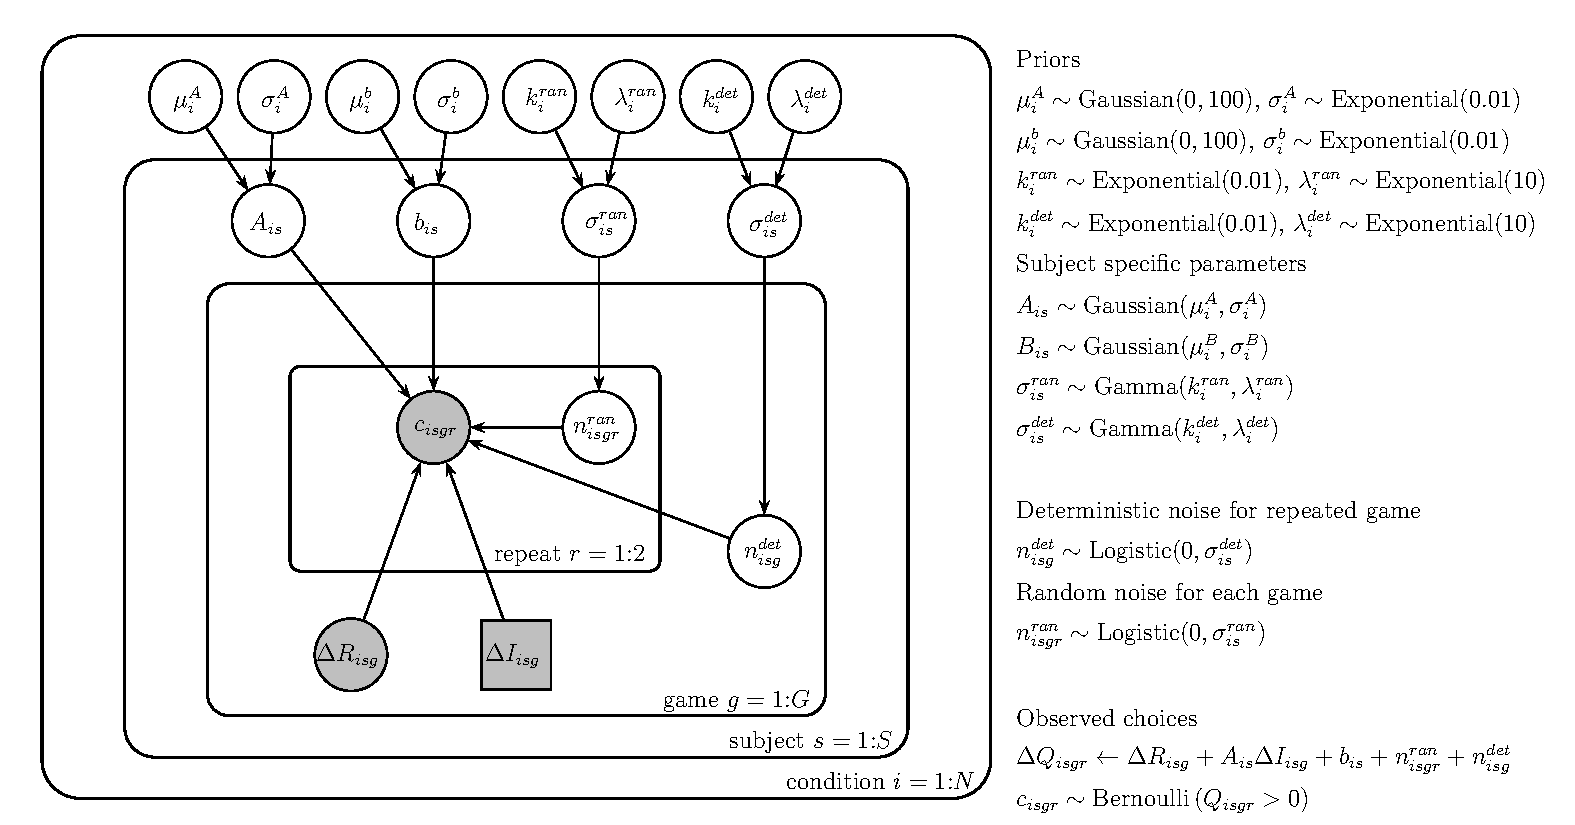
\includegraphics[width=1\textwidth]{figures/EEHorizon_2sigma.pdf}
\caption{Schematic of the hierarchical Bayesian model using notation of \cite{lee_wagenmakers_2014}}
\label{fig:model}
\end{center}
\end{figure}

\subsection*{Data and code}
Behavioral data as well as MATLAB codes to recreate the main figures from this paper will be made available upon publication. %website at https://dataverse.harvard.edu/dataset.xhtml?persistentId=doi:10.7910/DVN/CZT6EE.


\bibliographystyle{plainnat}
%\bibliographystyle{unsrt}
\bibliography{Refs/refs}

% add the Bibliography to the Table of Contents
\cleardoublepage
\ifdefined\phantomsection
\phantomsection  % makes hyperref recognize this section properly for pdf link
\else
\fi
\addcontentsline{toc}{chapter}{Bibliography}


%\listofchanges

\end{document}
